%%%%%%%%%%%%%%%%%%%%%%%%%%%%%%%%%%%%%%%%%%%%%%%%%%%%%%%%%%%%%%%%%%%%%%%%%%%%
% AGUtmpl.tex: this template file is for articles formatted with LaTeX2e,
% Modified July 2014
%
% This template includes commands and instructions
% given in the order necessary to produce a final output that will
% satisfy AGU requirements.
%
% PLEASE DO NOT USE YOUR OWN MACROS
% DO NOT USE \newcommand, \renewcommand, or \def.
%
% FOR FIGURES, DO NOT USE \psfrag or \subfigure.
%
%%%%%%%%%%%%%%%%%%%%%%%%%%%%%%%%%%%%%%%%%%%%%%%%%%%%%%%%%%%%%%%%%%%%%%%%%%%%
%
% All questions should be e-mailed to latex@agu.org.
%
%%%%%%%%%%%%%%%%%%%%%%%%%%%%%%%%%%%%%%%%%%%%%%%%%%%%%%%%%%%%%%%%%%%%%%%%%%%%
%
% Step 1: Set the \documentclass
%
% There are two options for article format: two column (default)
% and draft.
%
% PLEASE USE THE DRAFT OPTION TO SUBMIT YOUR PAPERS.
% The draft option produces double spaced output.
%
% Choose the journal abbreviation for the journal you are
% submitting to:

% jgrga JOURNAL OF GEOPHYSICAL RESEARCH
% gbc   GLOBAL BIOCHEMICAL CYCLES
% grl   GEOPHYSICAL RESEARCH LETTERS
% pal   PALEOCEANOGRAPHY
% ras   RADIO SCIENCE
% rog   REVIEWS OF GEOPHYSICS
% tec   TECTONICS
% wrr   WATER RESOURCES RESEARCH
% gc    GEOCHEMISTRY, GEOPHYSICS, GEOSYSTEMS
% sw    SPACE WEATHER
% ms    JAMES
% ef    EARTH'S FUTURE
% ea    EARTH AND SPACE SCIENCE
%
%
%
% (If you are submitting to a journal other than jgrga,
% substitute the initials of the journal for "jgrga" below.)

\documentclass[draft, ms]{agutex}   %draft, [ms]
% To create numbered lines:

% If you don't already have lineno.sty, you can download it from
% http://www.ctan.org/tex-archive/macros/latex/contrib/ednotes/
% (or search the internet for lineno.sty ctan), available at TeX Archive Network (CTAN).
% Take care that you always use the latest version.

% To activate the commands, uncomment \usepackage{lineno}
% and \linenumbers*[1]command, below:

\usepackage{lineno}
\linenumbers*[1]
%  To add line numbers to lines with equations:
%  \begin{linenomath*}
%  \begin{equation}
%  \end{equation}
%  \end{linenomath*}
%%%%%%%%%%%%%%%%%%%%%%%%%%%%%%%%%%%%%%%%%%%%%%%%%%%%%%%%%%%%%%%%%%%%%%%%%
\usepackage{url}
\usepackage{amsmath}
\usepackage{rotating} 

\usepackage{lineno}
\usepackage[bottom]{footmisc}

\usepackage{graphics}

%\usepackage[dvips]{graphicx}
 
\usepackage{color}
\definecolor{pinkred}{rgb}{1.0, 0.4, 0.4}

% Author names in capital letters:
\authorrunninghead{HUANG ET AL.}

% Shorter version of title entered in capital letters:
\titlerunninghead{HIGH-RESOLUTION REGIONAL CLIMATE MODEL EVALUATION}

%Corresponding author mailing address and e-mail address:
\authoraddr{Corresponding author: Xingying Huang,
Department of Land, Air and Water Resources, \\
 University of California Davis, Davis, CA 95616, USA.
 (xyhuang@ucdavis.edu)}
 
%Department of Hydrology and Water Resources, University of
%Arizona, Harshbarger Building 11, Tucson, AZ 85721, USA.
%(a.b.smith@hwr.arizona.edu)}

\begin{document}

%% ------------------------------------------------------------------------ %%
%
%  TITLE
%
%% ------------------------------------------------------------------------ %%


\title{High-resolution regional climate model evaluation using variable-resolution CESM over California}
%
% e.g., \title{Terrestrial ring current:
% Origin, formation, and decay $\alpha\beta\Gamma\Delta$}
%

%% ------------------------------------------------------------------------ %%
%
%  AUTHORS AND AFFILIATIONS
%
%% ------------------------------------------------------------------------ %%

%Use \author{\altaffilmark{}} and \altaffiltext{}

% \altaffilmark will produce footnote;
% matching \altaffiltext will appear at bottom of page.

% \authors{A. B. Smith,\altaffilmark{1}
% Eric Brown,\altaffilmark{1,2} Rick Williams,\altaffilmark{3}
% John B. McDougall\altaffilmark{4}, and S. Visconti\altaffilmark{5}}

%\altaffiltext{1}{Department of Hydrology and Water Resources,
%University of Arizona, Tucson, Arizona, USA.}

%\altaffiltext{2}{Department of Geography, Ohio State University,
%Columbus, Ohio, USA.}

%\altaffiltext{3}{Department of Space Sciences, University of
%Michigan, Ann Arbor, Michigan, USA.}

%\altaffiltext{4}{Division of Hydrologic Sciences, Desert Research
%Institute, Reno, Nevada, USA.}

    \authors{Xingying Huang,\altaffilmark{1}
  Alan M. Rhoades, \altaffilmark{1} Paul A. Ullrich, \altaffilmark{1} 
  Colin M. Zarzycki, \altaffilmark{2}}

\altaffiltext{1}{Department of Land, Air and Water Resources, University of California, Davis}
\altaffiltext{2}{National Center for Atmospheric Research}


%%%%%%%%%%%%%%%%%%%%%%%%%%%%%%%%%%%%%%%%%%%%%%%%%%%%%%%%%%%%%%%%%%%%%
% ABSTRACT
%
% Enter your Abstract here

\begin{abstract}
%Understanding the effect of climate change at regional scales remains a topic of intensive research. Due to computational constraints, the fine horizontal resolutions required to reach these scales have been largely out of reach for current global climate models. However, high resolution is needed to represent fine-scale processes and topographic forcing, which are significant drivers of local climate variability. Although regional climate models (RCMs) have been widely used at these scales, variable-resolution global climate models (VRGCMs) have arisen as an alternative for studying regional weather and climate. 

In this paper the recently developed variable-resolution option within the Community Earth System Model (VR-CESM) is assessed for long-term regional climate modeling of California at $\sim$28 km and $\sim$14 km horizontal resolutions. The mean climatology of near-surface temperature and precipitation is analyzed and contrasted with reanalysis, gridded observational datasets and a traditional regional climate model (RCM) -- the Weather Research and Forcasting (WRF) model. Statistical metrics for model evaluation and tests for differential significance have been extensively applied. With only prescribed sea surface temperatures, VR-CESM tended to produce a warmer summer (by about 1 to 3 $^\circ$C) and overestimated overall winter precipitation (about 25$\%$-35$\%$) compared to reference datasets. Increasing resolution from 28 km to 14 km did not produce a statistically significant improvement in the model results. By comparison, the analogous WRF climatology (constrained laterally and at the sea surface by ERA-Interim reanalysis) was $\sim$1 to 3 $^\circ$C colder than the reference datasets, underestimated precipitation by $\sim$20$\%$-30$\%$ at 27 km resolution and overestimated precipitation by $\sim$65-85$\%$ at 9 km.  Overall, VR-CESM produced comparable statistical biases to WRF in key climatological quantities.  This assessment highlights the value of variable-resolution global climate models (VRGCMs) in capturing fine-scale atmospheric processes, projecting future regional climate and addressing the computational expense of uniform-resolution global climate models.

\end{abstract} 

%Over the 26 years of historical climate simulations, VR-CESM adequately represent regional climatological patterns with high spatial correlations ($>$0.94) as WRF. 
%Higher resolution simulation of VR-CESM does produce better results in capturing summer maximum temperature and precipitation, along with their variability, than the coarser resolution run. However, the improvements are not statistically significant. 
%and a uniform high-resolution CESM with the finite volume (FV) dynamical core

\begin{article}

%%%%%%%%%%%%%%%%%%%%%%%%%%%%%%%%%%%%%%%%%%%%%%%%%%%%%%%%%%%%%%%%%%%%%
% MAIN BODY OF PAPER
%%%%%%%%%%%%%%%%%%%%%%%%%%%%%%%%%%%%%%%%%%%%%%%%%%%%%%%%%%%%%%%%%%%%%
%
\section{Introduction}

Global climate models (GCMs) have been widely used to simulate both past and future climate. Although these models have demonstrable success in representing large-scale features of the climate system, they are usually employed at relatively coarse resolutions ($\sim$1$^\circ$), largely as a result of the substantial computational cost required at higher resolutions. Global climate reanalysis datasets, which assimilate climate observations using a global model, represent a best estimate of historical weather patterns. However, reanalysis datasets still cannot fulfill the needs of policymakers, stakeholders and researchers that require high-resolution regional climate data (\url{http://reanalyses.org/atmosphere/overview-current-reanalyses}). Regional features such as microclimates, land cover, and topography, are not well captured by either GCMs or reanalysis datasets \citep{leung2003regional}.  However, dynamical processes at unrepresented scales are significant drivers for local climate variability, especially over complex terrain \citep{soares2012wrf}. In order to capture fine-scale dynamical features, high horizontal resolution is needed for a more accurate representation of small-scale processes and interactions \citep{rauscher2010resolution}. With these enhancements, regional climate data is expected to be more useful for formulating climate adaptation and mitigation strategies locally.

%{\color{red} CFSR is finer than this resolution. ~38km, no finer than 0.25$^\circ$ } 

In order to model regional climate at high spatial resolutions over a limited area, downscaling techniques have been developed, such as statistical and dynamical downscaling. Dynamical downscaling typically uses nested limited-area models (LAMs) or, more recently, variable-resolution enabled GCMs (VRGCMs) \citep{laprise2008regional}. In this context, LAMs are typically referred to as regional climate models (RCMs) when used for climate study. Forced by the output either from GCMs or reanalysis datasets, RCMs have been widely used to capture physically consistent regional and local circulations at the needed spatial and temporal scales \citep{christensen2007regional, bukovsky2009precipitation, mearns2012north}. Recently, there has been a growing interests in the use of VRGCMs for modeling regional climate. Unlike RCMs, VRGCMs use a relatively coarse global model with enhanced resolution over a specific region \citep{staniforth1978variable, fox1997finite}.  Strategies that have been employed for transitioning between coarse and fine-resolution regions within a VRGCM include grid stretching \citep{fox1997finite, mcgregor2008updated} and grid refinement \citep{ringler2008multiresolution, skamarock2012multiscale, zarzycki2014aquaplanet}. VRGCMs have been demonstrated to be effective for regional climate studies and applications at a reduced computational cost compared to uniform GCMs \citep{fox2006variable, rauscher2013exploring, zarzycki2015effects}. 

%fox2001variable, 
%\cite{fox2000uniform} found that the stretched-grid version of a GCM not only captured large-scale meteorological patterns but also mesoscale features, particularly those associated with orographic forcing.

%\citep{fox1997finite, ringler2008multiresolution, skamarock2012multiscale}
%The first is statistical downscaling, which aims to estimate fine scale behavior via analysis of the statistical relationships between observed small-scale variables and larger (GCM) scale variables \citep{fowler2007linking}. This method is empirical and cannot be used if the observed relationships do not hold under a changing climate. Dynamical downscaling, which uses a numerical model to simulate higher spatial resolution conditions in greater detail. 

Compared with RCMs, a key advantage of VRGCMs is that they use a single, unified modeling framework, rather than two separate models (GCM and RCM) with potentially disparate dynamics and physics parameterizations. RCMs may suffer from potential inconsistencies between the global and regional scales and lack two-way interactions at the nest boundary \citep{warner1997tutorial, mcdonald2003transparent, laprise2008challenging, mesinger2013limited}, which can be mitigated with the use of VRGCMs. VRGCMs also provide a cost-effective method of reaching high resolutions over a region of interest -- the limited area simulations in this study at 28km and 14km resolution represent a reduction in required computation of approximately 10 and 25 times, respectively, compared to analogous globally uniform high-resolution simulations. For the purposes of this paper, we focus on the recently developed Community Earth System Model with variable-resolution option (VR-CESM) as our VRGCM of interest. This configuration is driven by the Community Atmosphere Model's (CAM's) Spectral Element (SE) dynamical core, which possesses attractive conservation and parallel scaling properties \citep{dennis2011cam, taylor2011conservation}, as well as recently developed variable-resolution capabilities \citep{zarzycki2014aquaplanet}. This model has been employed by \cite{zarzycki2014using} to show that a high-resolution refinement patch in the Atlantic basin for simulating topical cyclones represented significant improvements over the unrefined simulation. \cite{zarzycki2015effects} also compared the large-scale climatology of VR-CESM 0.25$^\circ$ and uniform CESM at 1$^\circ$, and found that adding a refined region over the globe did not noticeably affect the global circulation. \cite{Rhoades2015Characterizing} has also assessed the use of VR-CESM for modeling Sierra Nevada mountain snowpack in the western United States.

%However, in order to obtain deeper insight into the performance of these two modeling approaches, it is necessary to compare them directly. 

However, for the purposes of long-term regional climate modeling, particularly in California, VR-CESM has yet to be rigorously evaluated. This paper aims to fill that gap by analyzing the performance of VR-CESM against gridded observational data, reanalysis data and in comparison to a traditional RCM.  Our variable-resolution simulations are implemented with horizontal resolutions of 28km and 14km respectively, which are much more typical for dynamically downscaled studies. This paper focuses on California in the western United States as the study area. With its complex topography, coastal influence, and wide latitudinal extent, California is an excellent test bed for regional climate modeling. Further, an understanding of local climate variability is incredibly important for policymakers and stakeholders in California due to its vast agricultural industry, mixed demographics, and vulnerability to anthropogenically-induced climate change \citep{hayhoe2004emissions, cayan2008overview}. 


For comparison, the Weather Research and Forecasting (WRF, \cite{skamarock2005coauthors}) model has been used for simulating California's climatology at 27km and 9km grid spacing. RCM simulations over California have also been conducted in previous studies and demonstrated the need for high spatial and temporal resolution to better address regional climate and extreme events, especially in the vicinity of complex topography where large climatological gradients are present \citep{leung2004mid, kanamitsu2007fifty, caldwell2009evaluation, pan2011influences, pierce2013probabilistic}. In particular, \cite{caldwell2009evaluation} presented results from WRF at 12km spatial resolution and showed that, although the RCM was effective at simulating the mean climate when compared with observations, some clear biases persisted (particularly an overestimation of precipitation).


This study focuses on the models' ability to represent current climate statistics, particularly those relevant to heat and precipitation extremes. We anticipate that this work will validate VR-CESM for modeling the mean regional climatology of California and will further motivate the adoption of variable-resolution modeling to study other local climatic processes. Our eventual goal is to utilize these models for assessing historical and future regional climate extremes.

%In addition, comparisons are drawn with a costly uniform high-resolution CESM simulation \citep{wehner2014resolution}. 



This paper is organized as follows: Section 2 describes the model setup, datasets and methodology for evaluation and intercomparison. In section 3, simulation results are provided and discussed, with focuses on near-surface (2-meter) temperature and precipitation. Key results are summarized along with further discussion in section 4.

%In almost all RCM studies, model precipitation was found to be overpredicted over the mountains of the west coast (a point discussed further in Section 3.1). Temperature biases seem to be more model dependent. Based on an intercomparison of 4 different RCM+GCM combinations, Duffy et al. (2006) also investigates model variances and precipitation- temperature correlation. 

%They should present the importance of studying California's climate at the beginning, which would make their objective more understandable. ???

%Among these studies, Kanamitsu et al. (2007) dynamically downscaled reanalysis data to 10-km resolution over CA showing the ability to study various regional climate phenomena within different time scales \citep{kanamitsu2007fifty}.

%paper: Exploring a Multi-resolution Approach Using AMIP Simulations_2015

\section{Models and Methodology}

\subsection{Simulation design} 

In this study, all global simulations use the Atmospheric Model Intercomparison Project (AMIP) experimental protocols \citep{Gates1992}. These protocols are widely used and support climate model diagnosis, validation and intercomparison. AMIP experiments are constrained by realistic sea-surface temperatures (SSTs) and sea ice from 1979 to near present without the added complexity of ocean-atmosphere feedbacks in the climate system. In particular, observed SSTs and sea ice at 1$^\circ$ horizontal resolution are provided and updated following the procedure described by \citep{hurrell2008new}.

%SSTs and ice coverage are supplied by the 1 $^\circ$ Hadley Centre Sea Ice and Sea Surface Temperature dataset (HadISST) \citep{hurrell2008new}. 

%{\color{red}attempt to recreate a climatology similar to that observed over the past few decades [I don't think this is a good characterization]}
%It is not meant to be used for climate change prediction, an endeavor that requires a coupled atmosphere-ocean model (e.g., see AMIP's sister project CMIP). http://www-pcmdi.llnl.gov/projects/amip/NEWS/overview.php

\subsubsection{VR-CESM}

CESM is a state-of-the-art Earth modeling framework managed by the National Center for Atmospheric Research (NCAR), consisting of coupled atmospheric, oceanic, land and sea ice models.  For decades CESM has been used for modeling present and future global climate \citep{neale2010description, hurrell2013community}.  The coupling infrastructure in CESM communicates the interfacial states and fluxes between each component model to ensure conservation. Since we follow AMIP protocols, only the atmosphere and land model are integrated dynamically. Here, CAM version 5 (CAM5) \citep{CAM5Tech} and the Community Land Model (CLM) version 4.0 \citep{CLM40Tech} are used. As mentioned earlier, the SE dynamical core is employed along with variable-resolution grid support. The FAMIPC5 (F$\_$AMIP$\_$CAM5) component set is chosen for these simulations.

For our study, the variable-resolution cubed-sphere grids are generated for use in CAM and CLM with the open-source software package SQuadGen \citep{ullrich2014squadgen,guba2014spectral}. The grids used in this study are depicted in Figure \ref{fig:VR-CESM_map}.  The maximum horizontal resolution on these grids is 0.25$^\circ$ ($\sim$28km) and 0.125$^\circ$ ($\sim$14km) respectively, with a quasi-uniform 1$^\circ$ mesh over the remainder of the globe. Grids are constructed using a paving technique with a 2:1 spatial resolution ratio, so two transition layers are required from 1$^\circ$ to 0.25$^\circ$, and one additional transition from 0.25$^\circ$ to 0.125$^\circ$. In our study, and previous studies (e.g. \cite{zarzycki2015effects}), general circulation patterns (e.g., wind, pressure and precipitation) do not exhibit apparent artifacts in the variable-resolution transition region, and the design of the SE dynamical core ensures that dry air and tracer mass are conserved globally \citep{taylor2010compatible}. Simulations are performed over the time period from 1979-01-01 to 2005-12-31 (UTC) and year 1979 is discarded as a spin-up period. This 26-year time period is chosen to provide an adequate sampling of inter-annual variability, to limit computational cost, and to coincide with the satellite era where adequate high-quality gridded and reanalysis datasets are available.

%The addition of a refined patch over the Atlantic basin does not noticeably affect the global circulation.
%How do fields near the refinement boundary look, as compared to uniform resolution? The 2 way interaction of WRF is not conserving, while the 1:2 refinement is conserving. This needs to be discussed and diagnostics near the boundary with respect to conservation done. In particular a comparison of point forecasts and climate averaging needs to be done, to investigate the deviation of the non conserving model and if the climate averaging takes this effect away.

Variable-resolution topography files were produced by sampling the National Geophysical Data Center (NGDC) 2-min ($\sim$4 km) Gridded Global Relief Dataset (ETOPO2v2), followed by the application of a differential smoothing technique as described in \cite{zarzycki2015effects}.  Using this technique, the $c$ parameter from their Eq. (1) was adjusted to reduce noise in the vertical pressure velocity field. The grid-scale topography is depicted in Figure \ref{fig:topo}, including the topography of uniform CESM at 1$^\circ$. As we can see, higher resolution provides clear improvement in the representation of regional topography, which is necessary for the correct treatment of fine-scale dynamic processes strongly influenced by complex terrain. Topography at very coarse resolution ($\sim$1$^\circ$) cannot represent local details like the shape of valleys or mountain peaks, resulting in the loss of regional climate patterns.

Land surface datasets, including plant functional types, at $0.5$$^\circ$ were adopted. Greenhouse gas (GHG) concentrations and aerosol forcings are prescribed based on historical observations. CAM and CLM tuning parameters are not modified from their default configurations.

%F_AMIP_CAM5 (FAMIPC5)  Description: AMIP run for CMIP5 protocol with cam5 
%{\color{red} \url{http://www.cesm.ucar.edu/experiments/cesm1.0/#rcp}}

%the time step for different resolutions

%CAM 30 vertical levels

%\subsubsection{Uniform CESM} 

%Output from a globally uniform CESM run at 0.25$^\circ$ spatial resolution is utilized for comparison. It helps us to see if variable-resolution CESM, which is at much lower computation cost than uniform one, can show comparable performance in modeling mean climatology \citep{bacmeister2014exploratory}. This globally uniform simulation uses the CAM5-FV (finite volume) dynamical core and is described in additional detail in \cite{wehner2014effect}. 

%{\color{red}I'm also not sure if uniform CESM should even be included. Maybe it should be removed. Huang: no info about CLM}

%Note that the appendix of the latter paper lists parameters that are different from the public release (i.e. the CAM5.1 default settings).

%The finest resolution considered in this study is based on a mesh of 0.23� by 0.31�. This resolution is still well suited to the hydrostatic approximation of the finite-volume dynamical core. However, it pushes the limits of the subgrid-scale parameterizations, particularly current representations of cumulus convective processes [Arakawa and Wu, 2013]. All three configurations in this study employ a standard 30 vertical level (L30) spacing scheme with a model top at approximately 2 hPa [Reed and Jablonowski, 2012]. Differences among select parameters employed for the three resolutions required by tuning and stability considerations are listed in Table A1 of Appendix Details of CAM5.1.

%Surface forcing of the atmospheric model is accomplished through prescribed sea surface temperatures and sea ice extent that follow the protocols of the Atmospheric Model Intercomparison Project (AMIP) [Gates, 1992; Gates et al., 1999]. These lower boundary conditions are available as part of the CESM public release. The integration and analysis period spans 1979�2005. At least one full year of integration was performed as a spin-up prior to this period and discarded for each resolution. In addition, the well-mixed greenhouse gases and both tropospheric and stratospheric ozone vary from year to year [Neale et al., 2010]. The aerosol forcing is also prescribed through external inputs since the default prognostic aerosol package was disabled in the interests of computational efficiency. This prescribed bulk aerosol formulation is as in CAM4 and designed to interact with the CAM5 cloud physics following Gettelman et al. [2008], adjusting sulfate activation so that drop number concentrations are similar to standard CAM5.1. All input forcing field files are available in the public release.

\subsubsection{WRF} 

WRF has been widely used over the past decade for modeling regional climate \citep{lo2008assessment, leung2009atmospheric, soares2012wrf, sun2015hybrid}. In our study, the fully compressible non-hydrostatic WRF model (version 3.5.1) with the Advanced Research WRF (ARW) dynamical core is used.  WRF is a limited area model that supports nested domains with a typical refinement ratio of 3:1.  The simulation domains of WRF are depicted in Figure \ref{fig:wrf_domains}. Two WRF simulations, representing finest grid resolutions of 27 km and 9 km, are conducted.  For the WRF 27km simulation, one domain is used. For the WRF 9km simulation, two domains are used, with the outer domain at 27 km (same as the WRF 27km) and an inner nested domain at 9 km horizontal grid resolution. For both simulations,  grids are centered on California and have 120$\times$110 and 151$\times$172 grid points, respectively. At all lateral boundaries, 10 grid points are used for relaxation to the coarse solution. In order to reduce the drift between forcing data and modeling output, grid nudging \citep{stauffer1990use} is applied to the outer domain every 6 hours at all levels except the planetary boundary layers (PBL), as suggested by \cite{lo2008assessment}. This setup uses 41 vertical levels with model top pressure at 50 hPa.

%Two-way nesting is enabled by overwriting coarse grid data by averaged fine grid data \citep{skamarock2008time} 

Additionally, the following physics parameterizations are employed: WSM (WRF Single-Moment) 6-class graupel microphysics scheme \citep{hong2006wrf}, Kain-Fritsch cumulus scheme \citep{kain2004kain}, CAM shortwave and longwave radiation schemes \citep{collins2004description}.  These settings are chosen by assessing the results from several common parameterization combinations over one-year simulation, with comparing to gridded observations. For the boundary layer, the Yonsei University scheme (YSU) \citep{hong2006new} is used, and the Noah Land Surface Model \citep{chen2001coupling} is applied. Both are chosen as they are common for climate applications that balance long-term reliability and computational cost.  Although many other options and combinations of parameterizations are available for configuring WRF (and others have tackled a complete assessment of these options for particular problems), our choices are made simply to represent a typical WRF configuration.

%(e.g. Grell-Freitas scheme) Grell et al. (2013); RRTM scheme (long wave)  Dudhia scheme (short wave)

ECMWF Reanalysis (ERA-Interim) data at both the surface and multiple pressure-levels provides initial and lateral conditions for the domains. The lateral conditions and SSTs are updated every 6 hours. ERA-Interim reanalysis ($\sim$80 km) has been widely used and validated for its reliability as forcing data \citep{dee2011era}. WRF simulations are conducted over the same time period as VR-CESM (i.e., 1979-01-01 through 2005-12-31 UTC). Again, the year 1979 is used as a spin-up period and is discarded for purposes of analysis. Notably, the $\sim$9 km resolution employed in the innermost domain is finer than most previous studies for long-term climate.

The topography employed for the 27 km and 9 km simulations is interpolated from USGS (United States Geological Survey) elevation data with 10-min ($\sim$20 km) and 2-min ($\sim$4 km) resolution, respectively. The post-processed grid-scale topography is contrasted in Figure \ref{fig:topo}. Elevation differences between VR-CESM and WRF are irregular and relatively small, except over the Central Valley where VR-CESM has consistently higher values than WRF. This indicates a different methodology for preparation of the topography dataset and may also be partly due to the use of the USGS elevation instead of NGDC elevation datasets. 

%{\color{red}Is there some quantitative assessment of these difference?  L2 difference?}.

%using all the meteorological and static data from nested domains as input.

%\subsection{Topography} 

\subsection{Methodology}

Near-surface temperature and precipitation have been analyzed over California to assess the performance of VR-CESM in representing the mean climatology. Specifically, our evaluation focuses on daily maximum, minimum and average near-surface temperatures (T$_{max}$, T$_{min}$ and T$_{avg}$) and daily precipitation (Pr). These variables are key in a baseline climate assessment due to their close relationship with water resources, agriculture and health. In this context, the biggest impact of weather on California is through heat and precipitation extremes. Since heat extremes dominate during the summer season, we focus on June, July and August (JJA) for assessment of temperature. On the other hand, since the vast majority of precipitation in California occurs in the winter season, December-January-February (DJF) is emphasized.  

%Future work will focus on the capability of the variable resolution system to correctly capture the features of discrete, extreme heat and precipitation events.

%Those seasons also represent the most of the climate variability.

In order to adequately account for natural variability of the mean climate, the simulation period must be chosen appropriately \citep{solomon2007climate}. However, the number of simulated years required for adequate climate statistics depends greatly on the regional climate variability and spatial scale. Past studies have used average weather conditions over a 30-year period to ensure sufficient statistics and to avoid imprinting from annual variability \citep{dinse2009climate}. To check that our 26-year simulation period is sufficient, we have examined the interannual variability of mean temperature and precipitation in all simulations and observations over 5, 10, 20 and 25 seasons or years. We observe that for climatological mean temperature and precipitation, the relevant statistics are effectively converged for a 20-year sample, suggesting that our simulation period is sufficient to adequately capture the variability of these quantities.

%adequately capturing the regionally climate variability. \textit{This is the type of vague wording the reviewers will attack us for.  Provide some quantification here.

% 30 years or longer run time may sound better, but are not necessary for our case.

The results in section 4 are obtained from simulated and observed data over the period 1980 to 2005.  All datasets have been linearly de-trended at each grid point so as to facilitate averaging of all simulation years. It is found that, for annual and JJA near-surface temperature (T$_{max}$, T$_{min}$ and T$_{avg}$), a statistically significant trend is present under the two-tailed t-statistic with a significance level of 0.05. The average magnitude of the linearly fit trend is about 1.3 K over 26 years for T$_{max}$, T$_{min}$ or T$_{avg}$. No statistically significant trend has been detected for precipitation.

%https://www.ncl.ucar.edu/Document/Functions/Built-in/regline.shtml
%https://www.ncl.ucar.edu/Document/Functions/Built-in/regCoef-1.shtml
%https://www.ncl.ucar.edu/Document/Functions/Built-in/cdft_p.shtml   %if the probability is larger than 0.975 at one-side, the null (rc=0) will be rejected at the significance level of 0.05. 
%https://www.ncl.ucar.edu/Document/Functions/Built-in/dtrend_msg_n.shtmll; without remove the mean
%However, the linear trend is week with linear regression coefficient averaged around 0.05.
%https://www.ncl.ucar.edu/Document/Functions/Built-in/dtrend.shtml  

California consists of a diverse variety of climate regions as a consequence of its rugged topography and large latitudinal extent.  The distinct character of these regions is poorly captured in typical coarse global climate simulations \citep{abatzoglou2009classification, caldwell2009evaluation}.  In order to assess the performance of VR-CESM within each region, the state has been divided into five climate divisions, including the Central Valley (CV), Mountain Region (MR), North Coast (NC), South Coast (SC), and Desert Region (DR).  The spatial extent of these divisions is depicted in Figure \ref{fig:wrf_domains}. These five divisions are determined loosely based on the results of \cite{abatzoglou2009classification} and the climate divisions used by the California Energy Commission. To restrict the analysis in each division, simulations and datasets have been masked to restrict climate variables to each division. 

Standard statistical measures have been used to quantify the model performance in comparison with the reference datasets. These include the root-mean-square deviation (RMSD), mean signed difference (MSD), mean relative absolute difference (MRD), and sample standard deviation ($s$). Further, spatial correlation is assessed by computing Pearson product-moment coefficient of linear correlation between climatological means from models and reference datasets.  Mathematically, these quantities are written as
\begin{align}
RMSD &= \sqrt{\frac{1}{N} \sum_{i=1}^{N} (v_i - \hat{v}_i)^2}  & MSD &= \frac{1}{N} \sum_{i=1}^{N} (v_i - \hat{v}_i) \\[2.0ex]
s &= \sqrt{\frac{1}{M-1} \sum_{j=1}^{M} (v_j - \bar{v})^2}   & MRD &= \left( \sum_{i=1}^{N} |v_i - \hat{v}_i| \right) \Bigg/ \left( \sum_{i=1}^{N} \hat{v}_i \right).
\end{align} where $v_i$ and $\hat{v}_i$ are values from the simulation output and reference dataset, respectively; $i$ is the grid-point index and N is the total number of grid points over specific regions; $j$ is the simulation year index, M is the total number of simulated years and $\bar{v}$ is the mean value over all years. Grid-point differences are calculated by remapping the reference datasets to the model's output grid using bilinear interpolation.  Remapping using patch-based interpolation has also been tested and nearly identical results have been observed.  When necessary, the statistical quantities are further averaged over each division.

%RMSD is defined as the square root of (the sum of the square difference (models-reference) over each grid point of the study area/(the numbers of the grid points)) (not N-1)
%MSD is defined as the mean signed difference (models-reference) over all these grid points
%MRD is defined as the mean relative absolute difference (sum (models-reference)/sum(reference)) over all these grid points
%sample standard deviation denoted by $s$, defined as the square root of (the sum of the square difference (x-xbar)/(the numbers of the size-1)), here the size are the number of years, the x is the value of each year for each grid point or averaged over each zone.

Throughout the remainder of this paper, student's t-test has been used to test whether two sets of annual-, seasonal- or monthly-average data are the same. F-test is applied to test whether the sample variances are equal. These tests are used only when the sample population can be described adequately by a normal distribution, where normality is assessed under the Anderson-Darling test. When the sample populations do not approximately follow a normal distribution, Mann-Whitney-Wilcoxon (MWW) test and Levene's test are employed in lieu of the t-test and F-test, respectively. All statistical tests are evaluated at the $p = 0.05$ significance level.

%{\color{red}It may be necessary to verify approximate normality when this test is applied} this can not can be done since the size is less than 100.

%T-test  for mean F-test for variability  under normal assumption when doing these test, the size do not -1 even using sample deviation
%http://stattrek.com/regression/slope-test.aspx?Tutorial=AP
%The significance level for a given hypothesis test is a value for which a P-value less than or equal to is considered statistically significant. Typical values for are 0.1, 0.05, and 0.01. These values correspond to the probability of observing such an extreme value by chance.
%t test: https://www.ncl.ucar.edu/Document/Functions/Built-in/ttest.shtml
%temp.R: for normal Test

%levene.test for variability under non-normal distribution (or any distribution); 
%Mann-Whitney-Wilcoxon test: http://www.r-tutor.com/elementary-statistics/non-parametric-methods/mann-whitney-wilcoxon-test

Complementary results to this study are provided in the online supplement, including the original grid-refined mesh files, the sensitivity of climatological statistics to choice of time period, the observed time trend, and other seasons not addressed in this paper and corresponding statistics metric tables. Results are also provided with comparison of VR-CESM to the output from a globally uniform CESM run at 0.25$^\circ$ spatial resolution with the finite volume (FV) dynamical core \citep{wehner2014effect}.

%, in order to see if variable-resolution CESM, which is at much lower computation cost than uniform one, can show comparable performance in modeling mean climatology \citep{bacmeister2014exploratory}

\subsection{Gridded and Reanalysis Datasets}

Reanalysis and gridded observational datasets of the highest available quality are employed (see Table \ref{tab:Datasets}). Differences between gridded observations can be due to the choice of meteorological stations, interpolation techniques, elevation models and processing algorithms.  Consequently, the use of multiple reference datasets is necessary to understand the underlying uncertainty in the observational data.  Detailed descriptions of these datasets are as follows.

%Although these products are employed to serve as realistic proxies for assessing the model results, we acknowledge that they may be sensitive to the choice of processing model and the set of assimilated observations and so cannot be treated as truth. 

%These data products incorporate station measurements or satellite information and other data. 

\paragraph{NARR}  The North American Regional Reanalysis (NARR) is the NCEP (National Centers for Environmental Prediction) high-resolution reanalysis product that provides dynamically downscaled data over North America at $\sim$32 km resolution and 3-hourly intervals from 1979 through present \citep{mesinger2006north}. We note that some inaccuracies have also been identified in NARR, particularly in precipitation fields \citep{bukovsky2007brief}.
%For this reason (and the relative coarseness of this product compared to gridded datasets) only temperature fields from NARR are used in this study.

%The NARR model uses the very high resolution NCEP Eta Model (32km/45 layer) together with the Regional Data Assimilation System (RDAS) which, significantly, assimilates precipitation along with other variables. (http://www.esrl.noaa.gov/psd/data/gridded/data.narr.html)

\paragraph{NCEP CPC} This dataset provides gauge-based analysis of daily precipitation from the National Oceanic and Atmospheric Administration (NOAA) Climate Prediction Center (CPC). It is a suite of unified precipitation products obtained by combining all information available at CPC via the optimal interpolation objective analysis technique. The gauge analysis covers the Conterminous United States with a fine-resolution at 0.25$^\circ$ from 1948-01-01 to 2006-12-31.

%CPC: National Oceanic and Atmospheric Administration (NOAA) uses more stations than University of Washington (UW); http://www.esrl.noaa.gov/psd/data/gridded/data.unified.daily.conus.html

\paragraph{PRISM} The Parameter-elevation Regressions on Independent Slopes Model (PRISM) \citep{daly2008physiographically} supports a 4 km gridded dataset obtained by taking point measurements and applying a weighted regression scheme that accounts for many factors affecting the local climatology. The datasets include total precipitation and minimum/maximum, (derived) mean temperatures and dewpoints. Monthly climatological variables are available for 1895 through 2014 from the PRISM Climate Group \footnote{Oregon State University, http://prism.oregonstate.edu, created 4 Feb 2004}. Notably, PRISM is the United States Department of Agriculture's official climatological dataset.  PRISM is used as our primary reference dataset for model performance evaluation.

\paragraph{UW} The UW daily gridded meteorological data is obtained from the Surface Water Modeling group at the University of Washington \citep{maurer2002long, hamlet2005production}. UW incorporates topographic corrections by forcing the long-term average precipitation to match that of the PRISM dataset. The temperature dataset is produced in a similar fashion as precipitation, but uses a simple 6.1 K/km lapse rate for topographic effect. The dataset is provided at 0.125$^\circ$ horizontal resolution covering the period 1949 to 2010.

%PRISM is a set of monthly, yearly, and single-event gridded data products of mean temperature and precipitation, max/min temperatures, and dewpoints, primarily for the United States.The PRISM products use a weighted regression scheme to account for complex climate regimes associated with orography, rain shadows, temperature inversions, slope aspect, coastal proximity, and other factors.  PRISM Ts, on the other hand, is based on a larger network of station data and accounts for elevation and topographic effects in a much more sophisticated manner. 

%the datasets I got have some small negative values (like -0.02 mm/d) for Pr. not sure why. Email PRISM about this.

\paragraph{Daymet}  Daymet is an extremely high resolution (1 km) gridded dataset with daily outputs of total precipitation, humidity, and minimum/maximum temperature covering 1980 through 2013 \citep{thornton1997generating, thornton2014daymet}. The dataset is produced using an algorithmic technique that ingests point station measurements in conjunction with a truncated Gaussian weighting filter.  Some adjustments are made to account for topography. Daymet is available through the Oak Ridge National Laboratory Distributed Active Archive Center (ORNL DAAC). 

%For applications of the radiation and humidity data please cite thornton1999improved, thornton2000simultaneous

To assess differences in these data products, we have calculated the MSD values among PRISM, UW and Daymet for seasonally averaged JJA T$_{max}$, T$_{min}$ and DJF Pr over the five divisions and tabulated these results in Table \ref{tab:stat_Datasets}. Student's t-test is employed to determine significances of differences. For T$_{max}$ and T$_{min}$, gridded observational datasets are different from each other over some divisions.  The most pronounced divergences occur in the NC region, with MSD values reaching up to $\sim$4$^\circ$C, although differences are also apparent for MR T$_{min}$. Clearly, UW and Daymet have a colder climatology than PRISM. NARR, as a reanalysis dataset, is different from the others over most divisions, with overall larger T$_{min}$ and smaller T$_{max}$. For precipitation, essentially no significant differences are present, especially among PRISM, UW and Daymet. NARR and CPC (not shown) seem to have slightly lower precipitation values than others.

%Those results further proved that uncertainty exists within these different products.

%pr DR SC ar not normal 
%Figure \ref{fig:obs_ttest}    as displayed in Figure \ref{fig:obs_ttest}
%

\section{Results}

\subsection{Temperature}

The mean JJA T$_{max}$, T$_{min}$ and T$_{avg}$ climatology over the simulation period, together with PRISM and NARR reference data, is plotted in Figure \ref{fig:t2_JJA}. UW and Daymet have not been plotted here since they are visually indistinguishable to PRISM everywhere except for NC, where UW and Daymet exhibit lower temperatures (see Table \ref{tab:stat_Datasets}).  Statistical measures over California are tabulated in Table \ref{tab:stat_JJA_t2}. In general, all simulations have captured the spatial climate patterns exhibited by PRISM, with high spatial correlations ($>$0.95), especially for T$_{max}$ and T$_{avg}$.  Nonetheless, several clear biases (relative to PRISM) are present in these simulations, as discussed below.

\begin{itemize}
\item{} \textbf{T$_{max}$:}  When compared with the reference datasets, VR-CESM showed a warm bias of about 2 to 3 $^\circ$C in T$_{max}$ over much of the inland domain (CV and MR) and a 2 to 3 $^\circ$C cool bias along the coast, although the coastal bias is reduced by $\sim$0.5 $^\circ$C at 14km resolution. This is in contrast with WRF, which produced an overall colder climate everywhere except the CV.  This bias is especially pronounced for the WRF 9km simulation, which was approximately 3 $^\circ$C cooler than PRISM. T$_{max}$ within the CV has been overestimated by all the simulations. This likely represents a systematic issue with high-resolution models with respect to California.  Possible reasons for this overestimation are discussed at the end of this section.

%Uniform CESM showed a similar outcome to VR-CESM, but with a larger RMSD value ($\sim$4$^\circ$C). 

\item{} \textbf{T$_{min}$:}  VR-CESM showed a strong warm bias in T$_{min}$ ($\sim$3 to 4 $^\circ$C), with a particularly large overestimation over Nevada ($> 5 ^\circ$C). WRF also exhibited a warm bias, but of a much smaller magnitude ($\sim$2 to 3 $^\circ$C). However, the pattern of T$_{min}$ presented in Figure \ref{fig:t2_JJA} in both WRF simulations suggests a cooler interior to the CV and warmer perimeter, which is not supported by observations.

\item{} \textbf{T$_{avg}$:}  The warm bias of T$_{min}$ and T$_{max}$ by VR-CESM resulted in a similar overestimation of T$_{avg}$. For WRF, underestimation of T$_{max}$ and overestimation of T$_{min}$ led to an overall closer match to T$_{avg}$ over most of the domain, but is indicative of a suppressed diurnal cycle.
\end{itemize}

Compared with the reference datasets over California, VR-CESM 0.125$^\circ$ produced the lowest RMSD values for T$_{max}$, whereas WRF had smallest RMSD for T$_{min}$.  However, in both cases the RMSD was around 2 $^\circ$C.  Notably, T$_{min}$ from VR-CESM matched much more closely with NARR, although this is likely indicative of a related warm bias in NARR.  In fact, closer examination of the differences among VR-CESM, WRF and NARR marine near-surface temperature patterns indicated that CESM and NARR have T$_{min}$ values that are approximately 2 $^\circ$C larger than WRF.  Since coastal near-surface temperature is strongly influenced by ocean SSTs, this difference is likely a key driver of the warm bias in CESM. The Delta breeze effect, which is associated with a sea breeze circulation that brings relatively cool and humid marine air into the interior CV from the San Francisco Bay area, was apparent in all runs. It is especially encouraging that VR-CESM generally performed as well as WRF, in comparison with reference datasets, even though VR-CESM was not constrained or nudged at the lateral boundaries of the high-resolution domain.

%Delta breeze a strong onshore atmospheric flow 

The spatial standard deviation of JJA T$_{max}$, T$_{min}$ and T$_{avg}$ from models and PRISM is presented in Figure \ref{fig:t2_JJA_std}. In PRISM, the CV had smaller variability than surrounding regions, although the difference is small ($\sim$0.2 $^\circ$C). Further, areas with rougher topography did exhibit somewhat higher variability than smoother locations. Interestingly, the higher resolution (0.125$^\circ$) VR-CESM simulation also matched the spatial pattern and magnitude of standard deviation observed in PRISM, especially for T$_{min}$ and T$_{avg}$. However, in WRF and VR-CESM 0.25$^\circ$, the variability is largely consistent across different divisions, and the values are around 0.5 to 1.5 $^\circ$C for all of the datasets, except for the high Sierras in the WRF 9km simulation which showed enhanced variability ($\sim$2 $^\circ$C). Compared with reference datasets, the RMSD values of VR-CESM and WRF 27km are $\sim$0.1-0.2 $^\circ$C, and $\sim$0.2-0.3 $^\circ$C for WRF 9km.

%Tmax>Tavg>Tmin
%From the RMSD values shown in Table \ref{tab:stat_std_JJA_t2}, VR-CESM and WRF 27km have smaller deviations ($\sim$0.1-0.2$^\circ$C) from observations comparing with WRF 9km ($\sim$0.2-0.3$^\circ$C).

%{\color{red}It would be interesting to calculate RMSE of the standard deviation. (done) A visual inspection suggests varres-0.125d has the best representation of variability.}

%can do the F-test for the standard deviation
%the t test of the JJA Tmax, T$_{min}$, T$_{avg}$ for cesm 0.25d and cesm 0.125d showed they have about half region is significantly the same at the level 0.05.
% (although difference are much smaller when focusing exclusively on California)

%However, these observations are still of the highest quality available and the uncertainty is relatively small compared with difference from the simulations. 
%VR-CESM overestimated all JJA temperatures (especially T$_{min}$), whereas WRF underestimates Tmax and T$_{avg}$.

%The RMSD values between the models and reference datasets range from $\sim$2 to 4$^\circ$C. It can still be seen that VR-CESM is comparable to WRF and uniform CESM, without meaning that they are statistically the same. 

%The DJF climatology is discussed here primarily due to its impact on snowpack. For Tmax (Figure \ref{fig:t2max_DJF}), all simulations show a warm bias over the Central Valley (that is especially pronounced for WRF 27 km), but a cold bias over almost all other regions (particularly in the mountain region of the WRF 9km simulations). For T$_{min}$ (Figure \ref{fig:t2min_DJF}), the model simulations show a warm bias over most regions except the mountain region. These errors were evidently smaller when comparing to PRISM rather than UW. For T$_{avg}$ (lower part of Figure \ref{fig:t2avg_JJA&DJF}), biases are quite smaller between models and PRISM dataset. Overall, the RMSDs are still roughly between 1 and 3 K, as noted in Table \ref{tab:stat_DJF_t2}, but were slightly reduced from summertime RMSDs. Simulations at coarser resolution seem to perform better overall, especially for VR-CESM 0.25$^\circ$ in Tmax, however, VR-CESM 0.25$^\circ$ shows largest error in modeling T$_{min}$. For VR-CESM, biases were largely unaffected by moving to higher resolutions, with a slight underprediction of Tmax and pronounced overprediction of T$_{min}$.  Moving to higher resolutions with WRF greatly increased biases in all cases.

The seasonal cycle of monthly mean T$_{avg}$ in each division is shown in Figure \ref{fig:trd_t2avg_allzones} for simulations and for reference data from PRISM and NARR along with the associated 95\% confidence interval. PRISM and NARR match closely almost everywhere except in the summer season of NC, SC and CV, indicative of underlying observational uncertainty. This difference is likely due to the discrepancy in assimilating the coastal cooling effect.  In general, model results match closely with reference data with no larger than a 2 $^\circ$C absolute difference, with the largest errors occurring in the summer and winter seasons.  Compared with PRISM, VR-CESM overpredicts summer T$_{avg}$ in all divisions except NC and SC, and underpredicts winter T$_{avg}$ in all divisions.  This corresponds to a larger annual temperature range. WRF has better performance in preserving the monthly trend when compared with CESM, with about 1 $^\circ$C underestimation over all seasons. There is no clear improvement in the seasonal cycle across resolutions.

%T test: WRF 27km is same as PRISM over most seasons over MR, VR-CESM is same as over spring and fall in MR, for CV, all are same over fall and winter, for DR, WRF is same as especially WRF 27km. fall and spring for VR-CESM, for SC, WRF is same except summer, for NC, all are different except part of the winter season

%There is as largest as $\sim$ 3$^\circ$C difference between NARR and PRISM over south coast during JJA, which may due to the assimilation of strong coastal cooling effect within NARR or the lack of enough in-field observations.

%Uniform CESM was similar to, but statistically different from VR-CESM, with a larger deviation of around 3$^\circ$C. 

%{\color{red}VR-CESM is different from WRF} based on the p value, Uniform-CESM is different from others.
%monthly values over 26 year pass the normal test except VR-CESM over north coast, so 95% confidence interval is given for reference datasets.

Variability in monthly average T$_{avg}$ is expressed by the interannual standard deviation of monthly T$_{avg}$ over the 26-year period and is plotted in Figure \ref{fig:trd_t2avg_allzones_std} for all divisions. Generally, standard deviation is between 1 to 2 $^\circ$C. Among all models, WRF 27km is closest to PRISM (when assessed using RMSD over the 12 month period). WRF 9km is also relatively close to PRISM, but exhibits an unusual $\sim$1 $^\circ$C increase in variability in January and February (statistically significant at the 0.05 level). VR-CESM exhibits a weaker correlation with PRISM in all divisions with enhanced variability in DJF and weakened variability in April and May at both resolutions, and in the fall season in the 0.125$^\circ$ simulation. Nonetheless, the standard deviation from all datasets is statistically equivalent to the reference (with $p > 0.05$), except for the WRF 9km results in January and February.

%{\color{red}[State which results are statistically significant]}

%all is the same as reference except WRF 9 over January to February. 

%Nonetheless, a comparison of these results using F-test indicated only these few statistically significant differences at the 95\% confidence level.

%showed that most of the variability values among these models do not have statistically significant differences.

%, and uniform CESM has about 0.5$^\circ$C lower variability than PRISM

%Due to the disorganized change of monthly variability, it is not easy to interpret this figure.

Due to the impact of summer heat waves, we now focus on T$_{max}$ over JJA. In Figure \ref{fig:PDF_t2max_allzones_JJA}, the frequency distribution of T$_{max}$ using all JJA daily values at each gridpoint over 26 years is depicted for models and reference data from UW and Daymet. PRISM is not included since it only deviates from UW and Daymet in the coastal divisions (NC and SC).  In these divisions PRISM is similar in character to UW but shifted several degrees towards warmer temperatures. Properties of the frequency distribution, including average, variability, skewness and Kurtosis are tabulated in Table \ref{tab:PDF_t2max_JJA}.  As exemplified by the similarity in the moments of the distribution, VR-CESM clearly captures the general distribution of T$_{max}$. Outside of the CV, skewness and kurtosis measures match closely between VR-CESM and the UW dataset. In the NC and SC, Daymet overestimates the frequency of very cold days leading to deviation in the moments from UW.  Consistent with the observations in Figure \ref{fig:t2_JJA}, outside of the CV, WRF tends to be cooler in general and VR-CESM tends to be warmer.  In NC and SC, all models more accurately capture the frequency of high T$_{max}$ days than low T$_{max}$ days. Enhanced frequency of cool T$_{max}$ values appears to be the primary driver in overestimation of sample variance in these divisions. For both VR-CESM and WRF there is no apparent improvement in statistics at higher resolutions.

%the p value of t2max pdf is all 0, so they are all different distributions. and their distribution did not pass the normality test.

In the CV, models show a clear warm bias and underestimated skewness, associated with a long forward tail and temperatures approaching near 50 $^\circ$C. As discussed earlier, all models overestimate T$_{max}$ over CV. In order to further assess the accuracy of the gridded observations, we examine the T$_{max}$ data directly from recorded weather station measurements over the CV (obtained from Global Historical Climate Network, provided by the NOAA/NCDC, \url{http://www.ncdc.noaa.gov/}). The results validate that T$_{max}$ values above 45 $^\circ$C are rare (although station observations suggest these days may be slightly more frequent than suggested by UW and Daymet). The warm bias associated with the aforementioned extreme hot days in both VR-CESM and WRF is likely correlated with overly dry summertime soil moisture, as discussed in \cite{caldwell2009evaluation}. This could be caused by the lack of accurate land surface treatment in climate models -- for example, \cite{bonfils2007empirical} found that irrigation in CV has significantly decreased summertime maximum temperatures, especially in heavily-irrigated areas. Other studies have also found the cooling effects of irrigation over CV, such as \cite{kueppers2007irrigation}.


%(0.14�C to 0.25�C per decade)

\subsection{Precipitation}

California's Mediterranean climate is associated with heavy precipitation in winter months and drier conditions in summertime.  Agricultural and urban water use in California thus depends on accumulation of wintertime precipitation, which accounts for approximately half of total annual average precipitation as we calculated.

%50 percent of the $\sim$22.5 inches that California receives for its total annual average precipitation amounts (\url{http://www.ncdc.noaa.gov/cag/}).

The long-term average climatology of DJF and annual daily Pr over 26 years from simulations and reference datasets (including PRISM and NARR) is depicted in Figure \ref{fig:pr_DJF_Anuual}. Other reference datasets are almost the same as PRISM. Statistical quantities over California are given in Table \ref{tab:stat_Pr}. We can see that precipitation is heavily influenced by orography, leading to most accumulation occurring along the NC and MR. As with temperature, the model results match the spatial patterns of the PRISM, with high correlation coefficients ($>$0.94).

%DJF is for 25 seasons

For DJF Pr, especially along the western edge of the Sierra Nevada and into the CV, VR-CESM overestimates total precipitation ($\sim$25$\%$-35$\%$) relative to PRISM (see MRD in Table \ref{tab:stat_Pr}), particularly for the coarser resolution (28 km) simulation. This difference is statistically significant over the western edge of the Sierra Nevada compared to PRISM at the 95\% level for VR-CESM 0.25$^\circ$. VR-CESM 0.125$^\circ$ performs better and produces far more realistic (and less scale sensitive) precipitation over the Sierra Nevada with improved treatment of orographic effects. On the other hand, precipitation is slightly underestimated relative to PRISM along the NC (with a statistically significant difference), particularly near the Oregon border. There are also notable differences between WRF 27km and WRF 9km that suggest a strong resolution dependence in the underlying microphysics. For DJF Pr, WRF 27km underestimates precipitation along the NC (by about 20$\%$-30$\%$), but fairly accurately captures precipitation in the CV; whereas WRF 9km greatly overestimates precipitation (by about 65$\%$-85$\%$) along the NC and MR (see MRD in Table \ref{tab:stat_Pr}). Using Table \ref{tab:stat_Pr} as a guide, VR-CESM 0.125$^\circ$ performs  better than VR-CESM 0.25$^\circ$ and WRF 27km with RMSD values around 1.2 mm$/$day over DJF. Since we expect most of this improvement is due to a better representation of topography at 14km, this result suggests that the default physical parameterization suite in CESM is fairly resolution insensitive. WRF 9km is significantly different from PRISM over the MR and part of NC, and the potential reasons are discussed at the end of this section. 

%For DJF Pr, especially along the western edge of the Sierra Nevada and into the CV, VR-CESM overestimates total precipitation ($\sim$25$\%$-35$\%$) relative to PRISM (see MRD in Table \ref{tab:stat_Pr}), particularly for the coarser resolution (28 km) simulation. This difference is statistically significant over the western edge of the Sierra Nevada compared to PRISM at the 95\% level for VR-CESM 0.25$^\circ$. VR-CESM 0.125$^\circ$ performs better and produces far more realistic (and less scale sensitive) precipitation over the Sierra Nevada with improved treatment of orographic effects. On the other hand, precipitation is slightly underestimated relative to PRISM along the NC (with a statistically significant difference), particularly near the Oregon border.

%There are also notable differences between WRF 27km and WRF 9km that suggest a strong resolution dependence in the underlying microphysics. For DJF Pr, WRF 27km underestimates precipitation along the NC (by about 20$\%$-30$\%$), but fairly accurately captures precipitation in the CV; whereas WRF 9km greatly overestimates precipitation (by about 65$\%$-85$\%$) along the NC and MR (see MRD in Table \ref{tab:stat_Pr}). Using Table \ref{tab:stat_Pr} as a guide, VR-CESM 0.125$^\circ$ performs  better than VR-CESM 0.25$^\circ$ and WRF 27km with RMSD values around 1.2 mm$/$day over DJF.  Since we expect most of this improvement is due to a better representation of topography at 14km, this result suggests that the default physical parameterization suite in CESM is fairly resolution insensitive. WRF 9km is significantly different from PRISM over the MR and part of NC, and the potential reasons are discussed at the end of this section.

%In fact, VR-CESM 0.125$^\circ$ and WRF 27km are statistically equivalent to PRISM everywhere except over part of NC, where uncertainty also tends to be largest. 
%Colin: You may want to borrow a reference or two from Alan's paper to point out where this may be a benefit to using a global model with convective/microphysical parameterizations that may be less regionally sensitive, especially if one is interested in important quantities like seasonal snowpack and water availability.



%WRF 27km is significantly different from PRISM  over coastal region and eastern side of the mountain region. VR-CESM 0.25d is significantly different from PRISM  over CV region and part of north coast region. {\color{red}Models at coarser resolution did not show organized patterns of similarity [What do you mean?]}. %In general, the relatively notable differences from Figure \ref{fig:pr_DJF_Anuual} also result statistically significant difference. 

%Uniform CESM has slightly better results than VR-CESM 0.25$^\circ$, especially over the  western edge of the Sierra Nevada, with about 10$\%$ reduced MRD values. 
%We can notice from the table that results are different when comparing \ref{tab:stat_Pr} that CPC with coarser resolution is not as consistent as other three observations.

Interannual variability of precipitation was calculated for the models and PRISM using the standard deviation of annual and DJF precipitation and depicted in Figure \ref{fig:pr_DJF_Annual_std}. In general, precipitation variability exhibits a similar pattern to the precipitation intensity. The spatial pattern of variability agrees well between models and PRISM, with the closest match provided by VR-CESM 0.125$^\circ$ and WRF 27km. Standard deviation is $\sim$50$\%$ higher for WRF 9km, consistent with overestimated precipitation intensity. VR-CESM 0.25$^\circ$ also tends to overestimate variability in the southern Sierra Nevada, likely due to over enhanced orographic uplift from the relatively coarse topography (relative to 0.125$^\circ$). Comparing with all the gridded observations, RMSD values are $\sim$0.7-0.9 mm$/$day for VR-CESM, $\sim$0.5-0.7 mm$/$day for WRF 27km, and $\sim$1.7-2.0 mm$/$day for WRF 9km.

%(as proved by Table \ref{tab:stat_Pr_std})

The annual cycle of precipitation averaged over each month and region for the models and reference datasets (taking PRISM and NARR as representative of all datasets) is presented in Figure \ref{fig:trd_pr_allzones}. The 95\% confidence intervals of UW and PRISM are also depicted; differences between models and reference datasets are statistically significant when simulation results appear outside of the highlighted region. In general, the overall monthly climatology is consistent between models and reference datasets, with highest precipitation values occurring over winter and lowest values over summer. Nonetheless, the largest deviations occur during the winter season. WRF 27km is drier than PRISM and UW with relative differences ranging from $\sim$10$\%$-40$\%$, whereas WRF 9km is far wetter with relative differences reaching up to 40$\%$-80$\%$ over these five divisions. VR-CESM tracks well with observed precipitation with $\sim$10$\%$-20$\%$ relative difference everywhere except in the CV, where precipitation is overestimated at rainy seasons with about 70$\%$-80$\%$. From the MWW test, VR-CESM and WRF 27km are not significantly different from reference datasets in most divisions, except over the CV in late winter to spring for VR-CESM 0.25$^\circ$, and the NC winter and spring, and DR's winter for WRF 27km. The magnitude of precipitation in WRF 9km is significantly different from the reference datasets over most divisions, except DR and SC's winter and spring. Nonetheless, the strong seasonal dependence on precipitation is apparent with extremely dry conditions during summer months. A slight increase in summertime precipitation is apparent in the DR, indicating the North American monsoon. However, we also observe that the peak month for precipitation tends to occur earlier in VR-CESM, particularly at 0.125$^\circ$, compared with the reference. VR-CESM also exhibits some unexpected jaggedness (particularly December for VR-CESM 0.25$^\circ$ and February for VR-CESM 0.125$^\circ$), likely due to an issue with capturing the seasonality of moisture transport over the Pacific. This issue being driven by variability outside of the high resolution domain seems corroborated by the observation that WRF correlates strongly with the reference datasets (even though the reported magnitude is incorrect).


%From the MWW test, the VR-CESM, uniform-CESM and WRF 27 is not different from reference datasets in major rainy regions especially over rainy seasons.

%no pattern for which p value is larger than which
%all p values results are mainly for rainy seasons
%Overall, VR-CESM is {\color{red}more close to} observations with smaller difference than WRF.

The monthly cycle of sample standard deviation is depicted in Figure \ref{fig:trd_pr_allzones_std}. The variability in observations has a similar monthly trend as precipitation rate, with overall values from 0 to 4 mm$/$day.  Generally, higher interannual variability occurs over locations with higher mean precipitation (see Figure \ref{fig:trd_pr_allzones}), also observed by previous studies (for example, \cite{duffy2006simulations}). Compared with observations, VR-CESM and WRF27km exhibited no more than 1 mm$/$day larger variability in the rainy season except over the CV. WRF 9km again showed enhanced variability ($\sim$1.5 mm$/$day more) during the wintertime over most divisions. The main cause of the interannual variability of precipitation over California is the El Ni\~{n}o-Southern Oscillation (ENSO), which varies the amount of moisture flux transported to this region. To assess deviations from observations, the Levene test was used in place of the F-test due to non-normality of precipitation. Under this test WRF 9km was significantly different from both reference datasets over summer and winter periods in MR, and over July to September in DR and SC.  VR-CESM 0.25$^\circ$ was significantly different within the CV over the  winter season.

%{\color{red}[January in the Desert?]}

%(except uniform CESM over south coast)

%The primary source of interannual variability in the study region is El Ni�o�Southern Oscillation (ENSO), which introduces variability primarily on times scales of 4 to 7 yr. This affects spatially averaged precipitation in the study region by varying the amount of moisture advected into the region.

The frequency distribution of DJF Pr has been constructed from rainy days (Pr$>$=0.1mm/day) for the simulations and reference datasets and depicted in Figure \ref{fig:PDF_pr_allzones_DJF}.  Since the frequency of precipitation is very similar across all reference datasets, only UW and CPC are included. Generally, VR-CESM matches closely with observations everywhere except in the CV. In the CV, WRF 27km appears to better capture high-intensity precipitation events, but performs poorly on low-intensity events (Pr$<$20 mm/day). The underestimation of rainfall frequency in WRF 27km appears consistent across divisions. WRF 9km produces a significantly better treatment of low-intensity events, but greatly overestimates the frequency of high-intensity events (Pr$>$20 mm/day). For strong precipitation events, VR-CESM matches closely to observations everywhere except the CV.

%Notably, VR-CESM 0.25 $^\circ$ and VR-CESM 0.125 $^\circ$ are not significantly different {\color{red}[give p-value of a two-sample K-S test]}. {\color{red}[give p-value of  a two-sample Kolmogorov-Smirnoff test]}

%the p value of DJF pr pdf is all 0 or far less than 0.05, so they are all different distributions. only at desert cpc and wrf27 showed 0.06.

%although these conclusions are also constrained by observational uncertainty {\color{red}[Should we even mention this given we can't quantify it?]}.

The overestimation of precipitation for WRF at high resolution has also been found in previous studies. Although not as pronounced as WRF 9km here, \cite{caldwell2009evaluation} demonstrated that WRF at 12km largely overestimated the precipitation over California's mountainous regions (however, this paper did employ a different set of parameterizations and had a different spatial extent of mountain region). Further discussion can be found in former studies that employ different microphysics schemes (and so produce a wide range of precipitation magnitudes) \citep{leung2003hydroclimate, jankov2005impact, gallus2006comparison, chin2010preliminary, caldwell2010california}. However, \cite{caldwell2009evaluation} also argued that the bias comes from a variety of sources, rather than simply different choices of sub-grid scale parameterizations. The exact cause of this overprediction has yet to be identified in the literature and a comprehensive analysis of the cause of these errors is beyond the scope of this paper. 

%, liu2011high , High-Resolution Simulations of Wintertime Precipitation in the Colorado Headwaters Region: Sensitivity to Physics Parameterizations
%Caldwell use CCSM output to force WRF and we are using ERA-Interim. And Caldwell "For this simulation, we prevent the regional model from drifting by reinitializing it from the GCM data on a monthly basis" rather than using nudging.

A concise summary of model performance for JJA near-surface temperature and DJF Pr over California is provided by the Taylor diagram (Figure \ref{fig:taylor_diagram}). This diagram includes the spatially centered correlation between the simulated and observed fields, the RMS variability of simulations normalized by that in the observations, and mean differences from a reference data \citep{taylor2001summarizing}. In general, all models correlate well with PRISM (used as the reference dataset in this diagram). As previously mentioned, WRF is better at modeling T$_{min}$ than VR-CESM; however, VR-CESM has smaller deviation for T$_{max}$. WRF 9km performs badly for precipitation with nearly a two times larger normalized standard deviation than other simulations. Overall, VR-CESM provides a competitive representation of the regional climatology over California and has errors which are comparable to WRF. Comparing resolutions, there is only minor improvement in VR-CESM 0.125$^\circ$ relative to 0.25$^\circ$ in simulating T$_{max}$ and Pr.

\section{Discussions and summary}

The need for high-resolution model data to address regional climate change and extreme events has motivated the development of new modeling tools.  Our study investigated the use of a variable-resolution GCM (i.e., VR-CESM) as an alternative approach for two-way dynamically downscaled climate modeling. The performance of VR-CESM was evaluated for modeling California's unique regional climate. This relatively new technique has been evaluated against gridded observational datasets, reanalysis data and the WRF model (forced with ERA-Interim data at lateral boundaries).

%To achieve this goal, uniform CESM is also included together with gridded reference datasets

Based on 26 years of high-resolution historical climate simulations (1980-2005), we analyzed the mean climatology of California across its climate divisions in terms of both near-surface temperature and precipitation. Generally, when compared with gridded observational datasets, both VR-CESM and WRF adequately represented regional climatological patterns with high spatial correlations ($>$0.94). Uncertainty between reference datasets exists, and is statistically significant over some climate divisions, making it necessary to utilize more than one high-quality observational products in the model evaluation. Overall, we found that VR-CESM showed comparable performance to WRF for regional climate modeling at spatial resolutions of 10-30 km.

%Even compared with a uniform high-resolution GCM (CESM-FV), VR-CESM also performed competitively.
%In the meantime, a uniform CESM simulation is also included. High-quality gridded datasets are used as reference datasets. 

Simulated temperature was assessed in terms of mean climatology of T$_{min}$, T$_{max}$ and T$_{avg}$ and interannual monthly-averaged variability of T$_{avg}$.  Deviations between the models and the reference datasets are apparent, but their character is different between VR-CESM and WRF. During the summer period, VR-CESM produced a 2 to 3 $^\circ$C warmer climate than observations, especially in the CV. On the other hand, WRF exhibited a colder ($\sim$2 $^\circ$C) T$_{max}$ over most divisions (except the CV), but was only a little warmer in T$_{min}$. Overall, VR-CESM was more accurate in reproducing mean climatology of T$_{max}$, whereas WRF was better at modeling T$_{min}$ and T$_{avg}$. WRF modeled the annual cycle of T$_{avg}$ better than VR-CESM with about a 1 $^\circ$C overall underestimation. VR-CESM overestimated T$_{avg}$ by 2 $^\circ$C over the summer season and underestimated T$_{avg}$ by 2 $^\circ$C over the winter season, indicating a larger annual temperature range over most divisions.

Temperatures were also assessed in terms of the climatology of JJA T$_{max}$, due to its relevance to summertime heat waves.  Both models successfully simulated the spatial character of JJA T$_{max}$, although both also had an apparent warm bias over the CV.  The failure to correctly capture CV T$_{max}$ is likely caused in part by the lack of irrigation cooling over this division in both models. Future work will address this issue by applying irrigation model to VR-CESM so as to figure out the role irrigation plays in regulating T$_{max}$ and its frequency distribution. Notably, the high-resolution (0.125$^\circ$) VR-CESM simulation accurately captured the spatial pattern of interannual variability for near-surface temperature when compared with PRISM. Both WRF and VR-CESM represented variability in monthly average T$_{avg}$ well over each climate division, except for the WRF 9km simulation in January and February where variability was greatly overestimated.

%For the frequency distribution of JJA T$_{max}$, both VR-CESM and WRF 27km matched closely to the UW dataset over all study areas except in the CV. 

%, and the overestimation and longer upbounded tail of frequency distribution for T$_{max}$

Precipitation was assessed in terms of mean climatology, interannual monthly-averaged variability and frequency of precipitation intensity.  In general, VR-CESM matched closely with PRISM everywhere except for an  overestimation of DJF Pr (about 25$\%$-35$\%$) along the western flank of the Sierra Nevada and into the CV. Increasing the spatial resolution to 0.125$^\circ$ produced some reduction in this overestimation (about 10$\%$) likely due to improved treatment of orographic effects. WRF 27km underestimated DJF precipitation (by about 20$\%$-30$\%$) along the NC and MR (where almost all the precipitation appears), whereas WRF 9km showed a large overestimation (about 65$\%$-85$\%$). The standard deviation of precipitation ranged from 0 to 6 mm$/$day, with generally higher interannual variability over locations of higher mean precipitation. When assessing the frequency of strong precipitation events, VR-CESM matched closely to the UW dataset everywhere except the CV.

%Our results also show that for these particular model configurations, VR-CESM is found to have a smaller resolution sensitivity with respect to precipitation in the Sierra Nevadas. This may be an advantageous result for multi-scale modelers interested in climate applications. Correctly simulating precipitation is vital to properly representing snowpack, which is of critical important to water availability in the western United States \citep{bales2006mountain, wise2012hydroclimatology, Rhoades2015Characterizing}. Decreased scale sensitivity implies a result will be more consistent, in magnitude, across a variety of grid spacings available to the regional modeler. 

%{\color{red}although the reference datasets also show some uncertainties [see earlier comment]}.

%with main deviation occurred during the rainy seasons. VR-CESM also exhibited a slightly larger variability than WRF 27km.  
%The main precipitation modeling deviations occurred during rainy seasons, especially in winter. 

Higher resolution (0.125$^\circ$) VR-CESM did produce better results when assessing JJA T$_{max}$ and precipitation (along with their variability), compared with the coarser resolution run. However, the improvements are not statistically significant over most of the study area.  The largest improvement at higher resolution was in the spatial character of precipitation, driven primarily with a better representation of the underlying topography. Notably, this result highlights the relative insensitivity to resolution in VR-CESM's physical parameterizations. This may be an advantageous result for multi-scale modelers interested in climate applications. Correctly simulating precipitation is vital to properly representing snowpack, which is of critical importance to water availability in the western United States \citep{bales2006mountain, wise2012hydroclimatology, Rhoades2015Characterizing}. Decreased scale sensitivity implies the result will be more independent of the choice of grid resolution. 

For WRF, when resolution is increased to 9km, the model produces vastly overestimated precipitation, as previous studies have also found when using RCMs for fine-scale regional simulations. Although the convective parameterization was not disabled (as is suggested for some models below 10km resolution), the effect of this change would likely not modify the results since almost all of the precipitation comes from resolved (large-scale) condensation (not shown). In this sense, precipitation modeling bias of WRF is more strongly related with resolved-scale processes and the choice of microphysics scheme plays a major role, motivating the need for more work on scale-aware parameterizations \citep{o2013observed}. 

%Since our grid spacing is approaching the 10 km bound beyond which subgrid-scale (commonly referred to as �convective�) parameterizations are perhaps not needed (e.g. Dudhia et al. 2003).

%The importance and necessity of high resolution for regional climate studies has been widely stressed by previous studies. However, whether the current regional climate models can fulfill this demand when resolution is pushed to regional scales is questionable. It is clear that further work is urgently needed to solve the scale limitation of current regional climate models at fine horizontal resolutions. The possible causes of the scale limitation may include a lack of accurate scare-aware physical parameterizations near or below 10 km horizontal resolution, the treatment of dynamics at fine scales, and the interactions among different components of RCMs or VRGCMs (e.g., land-atmosphere interactions). 

%A model�s performance can depend on horizontal resolution for different reasons: a more accurate representation of fine scale forcings (e.g. topography and land use), the better representation of processes and interactions (e.g. the dynamical structure of weather systems or cloud complexes; the location of major circulation features), and the direct dependence of physical parameterizations on the model grid size and time step interval.

In summary, VR-CESM demonstrated competitive utility for studying high-resolution regional climatology when compared to a regional climate model (WRF). Deviations exhibited within these models are not indicative of deep underlying problems with the model formulation, but one should nonetheless be aware of these biases when using these models for climate studies. This study suggests that VRGCMs are, in general, useful tools for assessing climate change over the coming century. As the need for assessments of regional climate change increases, alternative modeling strategies, including VRGCMs will be needed to improve our understanding of the effects of fine-scale processes representation in regional climate regulation. Future work will focus on the capability of the variable resolution system to correctly capture the features of discrete, extreme heat and precipitation events.

%and a uniform high-resolution GCM (CESM-FV)

%%%%%%%%%%%%%%%%%%%%%%%%%%%%%%%%%%%%%%%%%%%%%%%%%%%%%%%%%%%%%%%%%%%%%
% ACKNOWLEDGMENTS
%%%%%%%%%%%%%%%%%%%%%%%%%%%%%%%%%%%%%%%%%%%%%%%%%%%%%%%%%%%%%%%%%%%%%
\begin{acknowledgments}

%The authors would like to thank Michael Wehner and Da\'ith\'i Stone for providing the uniform resolution CESM dataset. 

The authors would like to thank Dr. Travis O'Brien for the many useful conversations on climate model assessment. We also want to thank Xue Meng Chen for her assistance in performing the WRF simulations. We acknowledge the work done to create the following datasets used in this study including PRISM, UW, Daymet, NARR and CPC (provided by the NOAA/OAR/ESRL PSD, Boulder, Colorado, USA, from their Web site at http://www.esrl.noaa.gov/psd/). This project is supported in part by the University of California, Davis and by the Department of Energy ``Multiscale Methods for Accurate, Efficient, and Scale-Aware Models of the Earth System'' program.
\end{acknowledgments}

\bibliographystyle{agufull08}
\bibliography{database2015}

\end{article}

%\section{Figures and tables}

% TABLES
\clearpage

%%%%%%%%%%%Table1%%%%%%%%%%%%%%%%%%%%%%%
\begin{table}
\caption{Reanalysis and gridded observational datasets used in this study.} \label{tab:Datasets}
\begin{center}
\begin{tabular}{lccccc} %{5in}{l @{\extracolsep{\fill}}cccc}
\hline \textbf{Data source} & \textbf{Variables used} & \textbf{Spatial resolution} & \textbf{Temporal resolution} \\
\hline \textbf{NARR} & Pr, T$_{s}$ & 32 km & daily, 3-hourly \\
\textbf{NCEP CPC} & Pr & $\sim$28 km (0.25$^\circ$) & daily \\
\textbf{UW} & Pr, T$_{min}$, T$_{max}$ & $\sim$14 km (0.125$^\circ$) & daily \\
\textbf{PRISM} & Pr, T$_{min}$, T$_{max}$, T$_{avg}$ & 4 km & monthly \\
\textbf{Daymet} & Pr, T$_{min}$, T$_{max}$ & 1 km & daily \\
\hline
\end{tabular}
\end{center}
\end{table}

%%%%%%%%%%%Table2%%%%%%%%%%%%%%%%%%%%%%%

\begin{table}
\caption{MSD (left column minus top row) of JJA temperature ($^\circ$C) and DJF precipitation (mm/day) between all reference datasets. Statistically significant differences are emphasized (95\% confidence level).} \label{tab:stat_Datasets}
\begin{tabular}{lccccccccccccccccc}
\hline \textbf{JJA T$_{min}$} & \multicolumn{5}{c}{\textbf{PRISM}} & & \multicolumn{5}{c}{\textbf{UW}} & & \multicolumn{5}{c}{\textbf{Daymet}} \\
\hline & MR &CV& DR& SC& NC & & MR& CV &DR &SC& NC & & MR &CV &DR &SC& NC \\
\hline \textbf{UW} & \textbf{\color{pinkred}-2.0} & \textbf{\color{pinkred}-0.5} & -0.3 & \textbf{\color{pinkred}-0.4} & \textbf{\color{pinkred}-2.3} \\
\textbf{Daymet} & \textbf{\color{pinkred}-1.8} & 0.2 & -0.2 & -0.3 & \textbf{\color{pinkred}-4.6} & & 0.2 & \textbf{\color{pinkred}0.8} & 0.1 & 0.1 & \textbf{\color{pinkred}-2.3} \\
\textbf{NARR} & \textbf{\color{pinkred}2.5} & \textbf{\color{pinkred}2.5} & \textbf{\color{pinkred}3.1} & -0.2 & \textbf{\color{pinkred}2.0} & & \textbf{\color{pinkred}4.5} & \textbf{\color{pinkred}3.1} & \textbf{\color{pinkred}3.4} & 0.2 & \textbf{\color{pinkred}4.2} & & \textbf{\color{pinkred}4.3} & \textbf{\color{pinkred}2.3 }& \textbf{\color{pinkred}3.2} & 0.1 & \textbf{\color{pinkred}6.5} \\
\hline \hline \textbf{JJA T$_{max}$} & \multicolumn{5}{c}{\textbf{PRISM}} & & \multicolumn{5}{c}{\textbf{UW}} & \multicolumn{5}{c}{\textbf{Daymet}} \\
\hline & MR &CV& DR& SC& NC & & MR& CV &DR &SC& NC & & MR &CV &DR &SC& NC \\
\hline \textbf{UW} & 0.3 & -0.1 & -0.2 & \textbf{\color{pinkred}-0.7} & \textbf{\color{pinkred}-2.4} \\
\textbf{Daymet} & -0.3 & 0.4 & -0.2 & 0.2 & \textbf{\color{pinkred}-3.7} & & -0.6 & \textbf{\color{pinkred}0.5} & 0.1 & \textbf{\color{pinkred}0.9} & \textbf{\color{pinkred}-1.3} \\
\textbf{NARR} & \textbf{\color{pinkred}-1.3} & \textbf{\color{pinkred}1.2} & -0.1 & \textbf{\color{pinkred}-0.6} & \textbf{\color{pinkred}-3.7} & & \textbf{\color{pinkred}-1.7} & \textbf{\color{pinkred}1.2} & 0.1 & 0.1 & \textbf{\color{pinkred}-1.3} & & \textbf{\color{pinkred}-1.1} & \textbf{\color{pinkred}0.7} & 0.1 & \textbf{\color{pinkred}-0.7} & 0.0 \\
\hline \hline \textbf{DJF Pr} & \multicolumn{5}{c}{\textbf{PRISM}} & & \multicolumn{5}{c}{\textbf{UW}} & & \multicolumn{5}{c}{\textbf{Daymet}} \\
\hline & MR &CV& DR& SC& NC & & MR& CV &DR &SC& NC & & MR &CV &DR &SC& NC \\
\hline \textbf{UW} & -0.2 & 0.1 & 0.0 & -0.2 & -0.2 \\
\textbf{Daymet} & -0.1 & -0.4 & -0.0 & 0.2 & 0.5 & & 0.1 & -0.5 & -0.0 & 0.3 & 0.8 \\
\textbf{NARR} & -0.5 & -0.4 & -0.1 & -0.1 &\textbf{\color{pinkred}-1.3} & & -0.3 & -0.5 & -0.1 & 0.1 & -1.1 & & -0.4 & -0.0 & -0.1 & -0.3 & \textbf{\color{pinkred}-1.8} \\ %& 0.2 $\ $ -0.5 $\ $ -0.1 $\ $ 0.0 $\ $ -0.2 \\
\textbf{CPC} & -0.8 & 0.0 & 0.0 & -0.1 & -1.1 & & -0.5 & -0.1 & 0.0 & 0.1 & -0.9 & & -0.6 & 0.4 & 0.0 & -0.3 & \textbf{\color{pinkred}-1.7} \\
\hline
\end{tabular}
\end{table}

%\begin{landscape}
%\begin{table}
%\caption{}
%\begin{center}

%\end{landscape}

% \begin{sidewaystable}
% \caption{}
% \begin{tabular}
% Table layout here.
% \end{tabular}
% \end{sidewaystable}

%%%%%%%%%%%%%%%%%%%%%%%%%%%%%%%%%%%%%%%
%\begin{table}
%\caption{MSD of JJA temperature and DJF precipitation between all reference datasets}
%\begin{center}

%
%%\begin{tabular}{lcccc}
%%\hline \textbf{T$_{avg}$} & \textbf{PRISM} \\
%%\hline & MR  $\ $ CV $\ $  DR $\ $  SC $\ $  NC \\
%%\hline \textbf{NARR} & 0.3 $\ $ {\color{red}1.6 $\ $ 1.6 $\ $ -1.0 $\ $ -1.4} \\
%%\hline 
%%\hline
%%\end{tabular}
%

%\tablenotetext{a}{

%%%%%%%%%%%Table3%%%%%%%%%%%%%%%%%%%%%%%
\begin{table}
\begin{center}
\caption{RMSD ($^\circ$C), MSD ($^\circ$C) and Spatial Correlation (Corr) for seasonally-averaged daily JJA temperatures over California. } \label{tab:stat_JJA_t2}
\begin{tabular*}{5.5in}{l @{\extracolsep{\fill}}ccccccccc}
\hline \textbf{RMSD} & \multicolumn{2}{c}{\textbf{UW}}  & & \multicolumn{3}{c}{\textbf{PRISM}} & & \multicolumn{2}{c}{\textbf{Daymet}} \\
\hline & T$_{max}$ &  T$_{min}$ & & T$_{max}$ & T$_{min}$ & T$_{avg}$& & T$_{max}$ & T$_{min}$\\
\hline \textbf{VR-CESM 0.25$^\circ$} & 2.32 & 3.75 & & 2.92 & 3.12 & 2.60 & & 2.81 & 3.93 \\
\textbf{VR-CESM 0.125$^\circ$} \quad & 1.90 & 3.63 & & 2.45 & 2.94 & 2.18 & & 2.48 & 3.70 \\
\textbf{WRF 27km} & 2.31 & 2.74 & & 2.93 & 2.25 & 2.17 & & 2.51 & 2.99 \\
\textbf{WRF 9km} & 3.32 & 2.94 & & 3.49 & 1.84 & 1.77 & & 3.20 & 2.94 \\
%\textbf{uniform CESM 0.25d} & 3.885 & 4.088 & 4.265 & 3.614 & 3.536 & 4.315 & 4.274 \\
\textbf{Uniform CESM 1$^\circ$} & 3.06 & 4.59 & & 3.62 & 3.43 & 3.16 & & 3.58 & 5.07 \\
\hline \hline \textbf{MSD} & \multicolumn{2}{c}{\textbf{UW}}  & \multicolumn{3}{c}{\textbf{PRISM}} & \multicolumn{2}{c}{\textbf{Daymet}} \\\hline & T$_{max}$ &  T$_{min}$ && T$_{max}$ & T$_{min}$ & T$_{avg}$&& T$_{max}$ &  T$_{min}$\\
\hline \textbf{VR-CESM 0.25$^\circ$} & 0.98 & 2.91 & & 0.61 & 1.73 & 0.82 & & 1.18 & 2.88 \\
\textbf{VR-CESM 0.125$^\circ$} \quad & 0.65 & 2.85 & & 0.20 & 1.66 & 0.58 & & 0.82 & 2.74 \\
\textbf{WRF 27km} & -0.58 & 0.82 & & -0.95 & -0.36 & -0.77 & & -0.39 & 0.79 \\
\textbf{WRF 9km} & -2.28 & 1.86 & & -2.72 & 0.67 & -1.14 & & -2.10 & 1.76 \\
%\textbf{uniform CESM 0.25d} & 1.812 & 2.993 & 1.449 & 1.815 & 1.280 & 2.013 & 2.961 \\
\textbf{Uniform CESM 1$^\circ$} & 0.82 & 3.03 & & 0.60 & 1.76 & 1.08 & & 1.24 & 3.38 \\
\hline \hline \textbf{Corr} & \multicolumn{2}{c}{\textbf{UW}}  & \multicolumn{3}{c}{\textbf{PRISM}} & \multicolumn{2}{c}{\textbf{Daymet}} \\\hline & T$_{max}$ &  T$_{min}$ && T$_{max}$ & T$_{min}$ & T$_{avg}$&& T$_{max}$ &  T$_{min}$\\
\hline \textbf{VR-CESM 0.25$^\circ$} & 0.99 & 0.98 & & 0.99 & 0.98 & 0.99 & & 0.99 & 0.97 \\
\textbf{VR-CESM 0.125$^\circ$} \quad & 0.99 & 0.98 & & 0.99 & 0.98 & 0.99 & & 0.99 & 0.98 \\
\textbf{WRF 27km} & 0.99 & 0.98 & & 0.99 & 0.98 & 0.99 & & 0.99 & 0.97 \\
\textbf{WRF 9km} & 0.99 & 0.98 & & 0.99 & 0.99 & 0.99 & & 0.99 & 0.98 \\
%\textbf{uniform CESM 0.25d} & 0.994 & 0.980 & 0.992 & 0.981 & 0.991 & 0.993 & 0.977 \\
\textbf{Uniform CESM 1$^\circ$} & 0.99 & 0.96 & & 0.99 & 0.97 & 0.99 & & 0.99 & 0.95 \\
\hline
\end{tabular*}
\end{center}
\end{table}


%%%%%%%Table4%%%%%%%%%%%%%%%%%%%%%%%%%%%%%%

%\begin{landscape}
\begin{table}
\caption{The first four moments of the JJA T$_{max}$ frequency in each climate division. Column titles refer to the Average (Avg), Variance (Var), Skewness (Skew) and Kurtosis (Kurt).} \label{tab:PDF_t2max_JJA}
\begin{tabular*}{5.0in}{l @{\extracolsep{\fill}}ccccccccc}
\hline \textbf{} & \multicolumn{4}{c}{\textbf{CV}}  & & \multicolumn{4}{c}{\textbf{MR}} \\
\hline & Avg &Var & Skew & Kurt & & Avg & Var & Skew & Kurt \\
\hline \textbf{UW} &32.6&	24.8	&-0.8&	0.9	& & 26.7	&33.2&	-0.4	&0.3 \\
\textbf{Daymet} & 32.7&	23.5&	-0.9&	1.5	& & 25.9	&39.3&	-0.5&	0.5	\\
\hline\textbf{VR-CESM 0.25$^\circ$}& 34.1&	26.2	&-0.4&	0.2	& & 28.1	&27.6&	-0.4&	0.3	\\
\textbf{VR-CESM 0.125$^\circ$}& 34.3	&28.5&	-0.5	&0.4	& & 27.2	&30.0&	-0.4&	0.3	\\
\hline\textbf{WRF 27km} & 33.9	&34.8	&-0.5&	0.2	& & 24.9	&34.8&	-0.3	&0.0	\\
\textbf{WRF 9km} & 32.4 &33.1	&-0.7&	0.6	& & 22.4		&38.5		&-0.5		&0.6	\\
\hline
\end{tabular*}

\begin{tabular*}{6.8in}{l @{\extracolsep{\fill}}cccccccccccc}
\hline \textbf{} & \multicolumn{4}{c}{\textbf{NC}} & \multicolumn{4}{c}{\textbf{SC}} & \multicolumn{4}{c}{\textbf{DR}} \\
\hline & Avg &Var & Skew & Kurt & Avg & Var & Skew & Kurt & Avg & Var & Skew & Kurt \\
\hline \textbf{UW} & 25.9	&30.4	&0.1&	-0.5		&25.9&	30.4	&0.1&	-0.5&		37.0	&22.9&	-0.6	&0.7\\
\textbf{Daymet} & 26.5	&30.1	&-0.3&	0.4	&	26.5	&30.1	&-0.3	&0.4		& 37.0	&24.3	&-0.6&	0.6\\
\hline\textbf{VR-CESM 0.25$^\circ$}& 26.4	&37.4	&0.1&	-0.7		& 26.4&	37.4	&0.1&	-0.7	&	37.6&	19.0&	-0.5	&0.8\\
\textbf{VR-CESM 0.125$^\circ$} & 26.3	&37.4&	0.1&	-0.6		& 26.3&	37.4&	0.1	&-0.6		& 37.3	&21.3&	-0.5	&0.4\\
\hline \textbf{WRF 27km} & 26.0	&36.7	&-0.1&	-0.5		& 26.0&	36.7	&-0.1	&-0.5		& 36.5&	22.6&	-0.6&	0.5\\
\textbf{WRF 9km} & 24.9 &32.6		&\,0.0		&-0.6	& 24.9&	32.6	&	0.0		&-0.6	&	34.4		&24.4		&-0.5		&0.4\\
\hline
\end{tabular*} \\

\begin{tabular}{p{6in}}
\small\textbf{Notes:} If skew $>0$ [skew $<0$], the distribution trails off to the right [left]. If kurtosis $> 0$ [$<0$], a sharper [flatter] peak compared to a normal distribution (leptokurtic and platykurtic, respectively) is expected.

\end{tabular}
\end{table}
%\end{landscape}
%%%%%%Table5%%%%%%%%%%%%%%%%%%%%%%%%%%%

%\begin{landscape}
\begin{table}
\begin{center}
\caption{RMSD (mm/day), MSD (mm/d), MRD, Spatial Correlation (Corr) for averaged precipitation over California} \label{tab:stat_Pr}
\begin{tabular*}{6.5in}{l @{\extracolsep{\fill}}cccccccccc}
%\resizebox{\textwidth}{!}
\hline \textbf{Annual} & \multicolumn{4}{c}{\textbf{CPC}}  & & \multicolumn{4}{c}{\textbf{UW}} \\
\hline $    $ & RMSD & MSD & MRD & Corr & & RMSD & MSD & MRD & Corr \\
\hline \textbf{VR-CESM 0.25$^\circ$} & 0.61 & 0.39 & 0.30 & 0.98 & & 0.62 & 0.29 & 0.29 & 0.96 \\
\textbf{VR-CESM 0.125$^\circ$} & 0.47 & 0.21 & 0.24 & 0.98 & & 0.53 & 0.12 & 0.24 & 0.97 \\
\textbf{WRF 27km} & 0.42 & -0.21 & 0.21 & 0.97 & & 0.58 & -0.31 & 0.24 & 0.97 \\
\textbf{WRF 9km} & 2.23 & 1.49 & 0.97 & 0.95 & & 2.05 & 1.39 & 0.85 & 0.96 \\
%\textbf{uniform CESM 0.25d} & 0.555 & 0.134 & 0.238 & 0.969 & 0.600 & 0.031 & 0.253 & 0.961 & 0.700 & -0.057 & 0.265 & 0.953 & 0.600 & -0.069 & 0.245 & 0.962 \\
\textbf{Uniform CESM 1$^\circ$} & 1.97 & -1.57 & 0.99 & 0.94 & & 2.31 & -1.70 & 0.99 & 0.91 \\
\hline & \multicolumn{4}{c}{\textbf{PRISM}} & \multicolumn{4}{c}{\textbf{Daymet}} \\
\hline $    $ & RMSD & MSD & MRD & Corr & & RMSD & MSD & MRD & Corr \\
\hline \textbf{VR-CESM 0.25$^\circ$} & 0.72 & 0.20 & 0.31 & 0.95 & & 0.57 & 0.19 & 0.25 & 0.97 \\
\textbf{VR-CESM 0.125$^\circ$} & 0.62 & 0.05 & 0.26 & 0.96 & & 0.50 & 0.03 & 0.22 & 0.97 \\
\textbf{WRF 27km} & 0.77 & -0.40 & 0.27 & 0.96 & & 0.65 & -0.41 & 0.27 & 0.97 \\
\textbf{WRF 9km} & 1.89 & 1.32 & 0.78 & 0.97 & & 2.01 & 1.31 & 0.76 & 0.96 \\
%\textbf{uniform CESM 0.25d} & 0.555 & 0.134 & 0.238 & 0.969 & 0.600 & 0.031 & 0.253 & 0.961 & 0.700 & -0.057 & 0.265 & 0.953 & 0.600 & -0.069 & 0.245 & 0.962 \\
\textbf{Uniform CESM 1$^\circ$} & 2.53 & -1.83 & 0.99 & 0.90 & & 2.31 & -1.80 & 0.99 & 0.93 \\
\hline
\
\end{tabular*}

\begin{tabular*}{6.5in}{l @{\extracolsep{\fill}}cccccccccc}
\hline \textbf{DJF} & \multicolumn{4}{c}{\textbf{CPC}} & & \multicolumn{4}{c}{\textbf{UW}} \\
\hline $    $ & RMSD & MSD & MRD & Corr & & RMSD & MSD & MRD & Corr \\
\hline \textbf{VR-CESM 0.25$^\circ$} & 1.49 & 0.99 & 0.36 & 0.97 & & 1.45 & 0.67 & 0.33 & 0.95 \\
\textbf{VR-CESM 0.125$^\circ$} & 1.19 & 0.64 & 0.29 & 0.97 & & 1.23 & 0.35 & 0.27 & 0.96 \\
\textbf{WRF 27km} & 0.89 & -0.38 & 0.21 & 0.97 & & 1.29 & -0.69 & 0.26 & 0.96 \\
\textbf{WRF 9km} & 4.26 & 2.61 & 0.86 & 0.95 & & 3.84 & 2.32 & 0.70 & 0.95 \\
%\textbf{uniform CESM 0.25d} & 1.392 & 0.377 & 0.286 & 0.960 & 1.431 & 0.064 & 0.283 & 0.951 & 1.544 & -0.033 & 0.293 & 0.946 & 1.406 & -0.095 & 0.275 & 0.953 \\
\textbf{Uniform CESM 1$^\circ$} & 3.97 & -3.12 & 0.99 & 0.93 & & 4.80 & -3.50 & 0.99 & 0.90 \\
\hline  & \multicolumn{4}{c}{\textbf{PRISM}} & \multicolumn{4}{c}{\textbf{Daymet}} \\
\hline $    $ & RMSD & MSD & MRD & Corr & & RMSD & MSD & MRD & Corr \\
\hline \textbf{VR-CESM 0.25$^\circ$} & 1.65 & 0.58 & 0.35 & 0.94 & & 1.35 & 0.51 & 0.28 & 0.96 \\
\textbf{VR-CESM 0.125$^\circ$} & 1.40 & 0.29 & 0.29 & 0.95 & & 1.17 & 0.21 & 0.25 & 0.96 \\
\textbf{WRF 27km} & 1.55 & -0.79 & 0.28 & 0.96 & & 1.35 & -0.85 & 0.28 & 0.96 \\
\textbf{WRF 9km} & 3.57 & 2.26 & 0.66 & 0.96 & & 3.80 & 2.18 & 0.65 & 0.95 \\
%\textbf{uniform CESM 0.25d} & 1.392 & 0.377 & 0.286 & 0.960 & 1.431 & 0.064 & 0.283 & 0.951 & 1.544 & -0.033 & 0.293 & 0.946 & 1.406 & -0.095 & 0.275 & 0.953 \\
\textbf{Uniform CESM 1$^\circ$} & 5.07 & -3.65 & 0.99 & 0.90 & & 4.69 & -3.65 & 0.99 & 0.93 \\
\hline
\
\end{tabular*}

\end{center}
\end{table}

\clearpage
%\end{landscape}
%%%%%%%%%%%%%%%%%%%%%%%%%%%%%%%%%%%%%%%%%%%%%%%%%%%%%%%%%%
%\begin{table}
%\begin{center}
%\caption{RMSD, Correlation (Corr) for precipitation over California} \label{tab:stat_Pr_std}
%\begin{tabular}{lcccc}
%\hline \textbf{Annual} & \textbf{CPC}  & \textbf{UW} & \textbf{PRISM} & \textbf{Daymet} \\
%\hline $    $ & RMSD $\ $ Corr & RMSD $\ $ Corr & RMSD $\ $ Corr & RMSD $\ $ Corr \\
%\hline \textbf{VR-CESM 0.25d} & 0.195 $\ $ 0.959 & 0.251 $\ $ 0.942 & 0.283 $\ $ 0.930 & 0.260 $\ $ 0.944 \\
%\textbf{VR-CESM 0.125d} & 0.203 $\ $ 0.969 & 0.233 $\ $ 0.954 & 0.245 $\ $ 0.950 & 0.220 $\ $ 0.959 \\
%\textbf{WRF 27km} & 0.159 $\ $ 0.974 & 0.209 $\ $ 0.968 & 0.228 $\ $ 0.964 & 0.236 $\ $ 0.963 \\
%\textbf{WRF 9km} & 0.742 $\ $ 0.953 & 0.686 $\ $ 0.961 & 0.668 $\ $ 0.968 & 0.679 $\ $ 0.956 \\
%\textbf{uniform CESM 0.25d} & 0.243 $\ $ 0.950 & 0.311 $\ $ 0.936 & 0.325 $\ $ 0.937 & 0.331 $\ $ 0.937 \\
%\hline
%\end{tabular}
%
%\begin{tabular}{lcccc}
%\hline \textbf{DJF} & \textbf{CPC}  & \textbf{UW} & \textbf{PRISM} & \textbf{Daymet} \\
%\hline $    $ & RMSD $\ $ Corr & RMSD $\ $ Corr & RMSD $\ $ Corr & RMSD $\ $ Corr \\
%\hline \textbf{VR-CESM 0.25d} & 0.788 $\ $ 0.932 & 0.851 $\ $ 0.917 & 0.924 $\ $ 0.904 & 0.801 $\ $ 0.927 \\
%\textbf{VR-CESM 0.125d} & 0.719 $\ $ 0.962 & 0.720 $\ $ 0.949 & 0.770 $\ $ 0.941 & 0.678 $\ $ 0.956 \\
%\textbf{WRF 27km} & 0.487 $\ $ 0.963 & 0.605 $\ $ 0.960 & 0.663 $\ $ 0.955 & 0.633 $\ $ 0.957 \\
%\textbf{WRF 9km} & 1.994 $\ $ 0.935 & 1.787 $\ $ 0.946 & 1.726 $\ $ 0.955 & 1.787 $\ $ 0.946 \\
%\textbf{uniform CESM 0.25d} & 0.707 $\ $ 0.921 & 0.861 $\ $ 0.908 & 0.892 $\ $ 0.907 & 0.834 $\ $ 0.916 \\
%\hline
%\end{tabular}
%\end{center}
%\end{table}

%%%%%%%%%%%%%%%%%%%%%%%%%%%%%%%%%%%%%%%%%%%%%%%%%%%%%%

%\subsection{Figures}

%Figure 1
\begin{figure}
\begin{center}
\includegraphics[width=6in]{worldmap_modified.pdf}
\caption{The approximate grid spacing in the (a) VR-CESM 0.25$^\circ$ and (b) VR-CESM 0.125$^\circ$ meshes used in this study. (c) A depiction of the transition from the global $1^\circ$ resolution mesh through two layers of refinement to $0.25^\circ$ and again to $0.125^\circ$.}
\label{fig:VR-CESM_map}
\end{center}
\end{figure}

%Approximate regional resolution for the computational grids used in VR-CESM simulations.  The dashed lines and solid lines correspond to the outer boundary and inner boundary of the transition region.

%Figure 2
\begin{figure}
\begin{center}
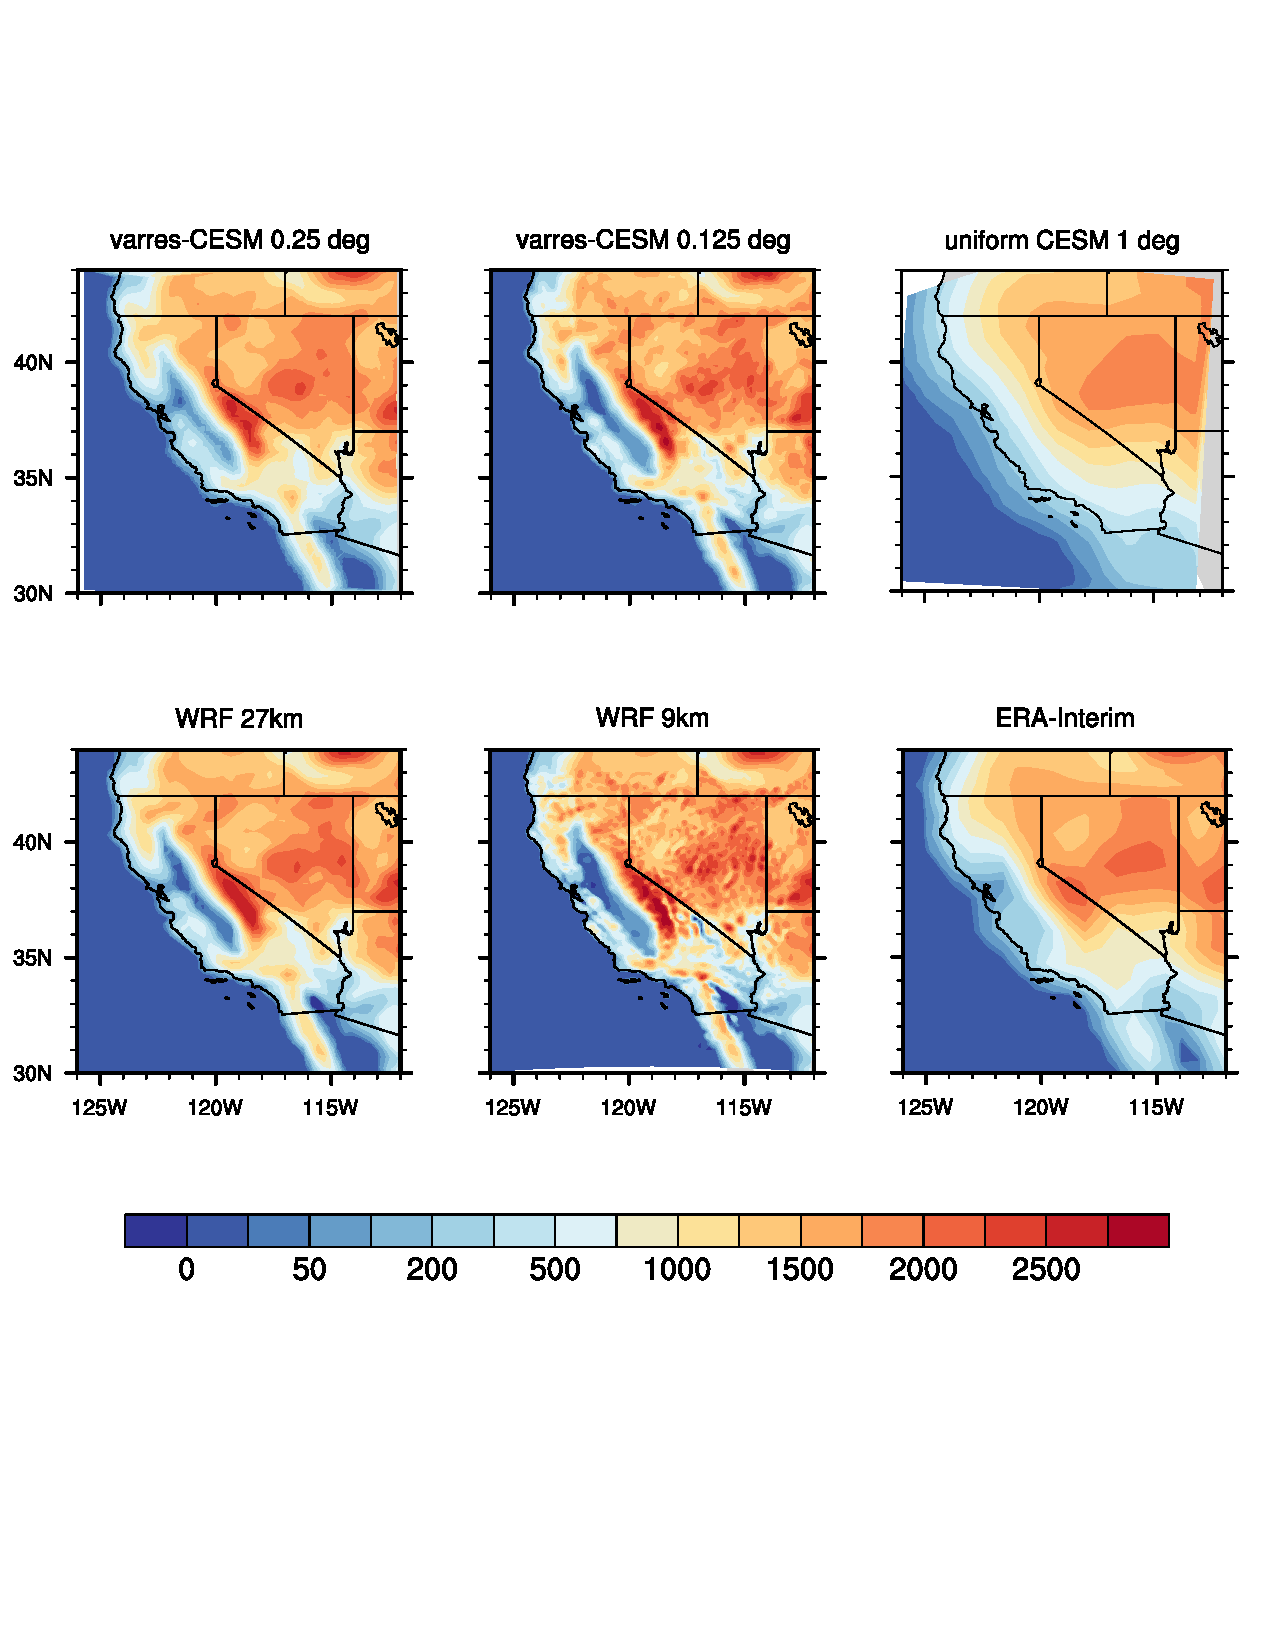
\includegraphics[width=6in]{topo.pdf}
\end{center}
\caption{Topographic heights (from top left to bottom right) for VR-CESM 0.25$^\circ$, VR-CESM 0.125$^\circ$, uniform CESM 1$^\circ$, WRF 27km, WRF 9km and ERA-Interim ($\Delta x \sim$80 km).} \label{fig:topo} 
\end{figure}

%Figure 3
\begin{figure}
\begin{center}
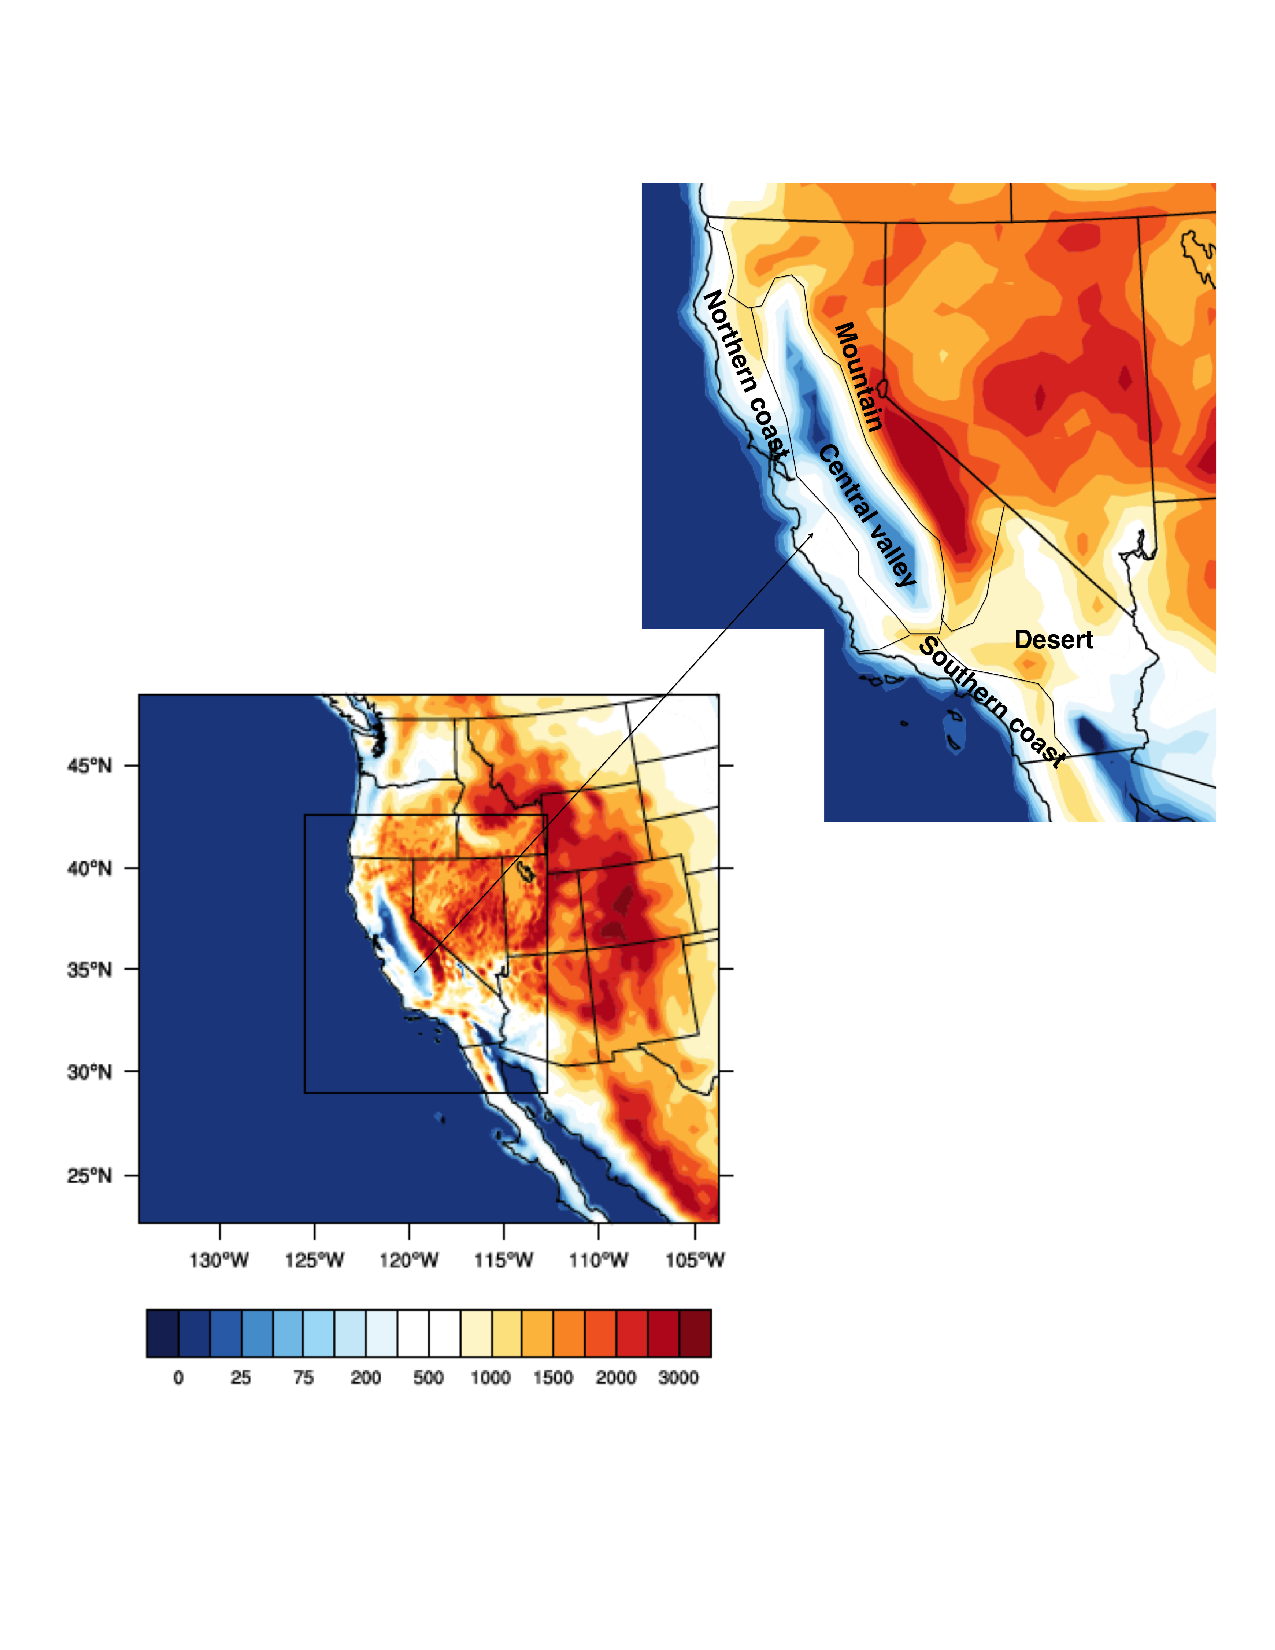
\includegraphics[width=6in]{wrf_domains.pdf}
\end{center}
\caption{Left: WRF 27km (entire plot region) and WRF 9km (solid black box) simulation domains; Right: five climate divisions for California.  Both plots are overlaid with WRF model topography.} \label{fig:wrf_domains}
\end{figure}

%\begin{figure}
%\begin{center}
%\inclu$^\circ$raphics[width=6in]{UW_PRISM_Daymet_ttest.pdf}
%\end{center}
%\caption{P values from the t-tests among UW, PRISM and Daymet datasets. Grids in green color are statistically significantly different from each other with p value less than 0.05.} \label{fig:obs_ttest} 
%\end{figure}

%Figure 4
\begin{figure}
\begin{center}
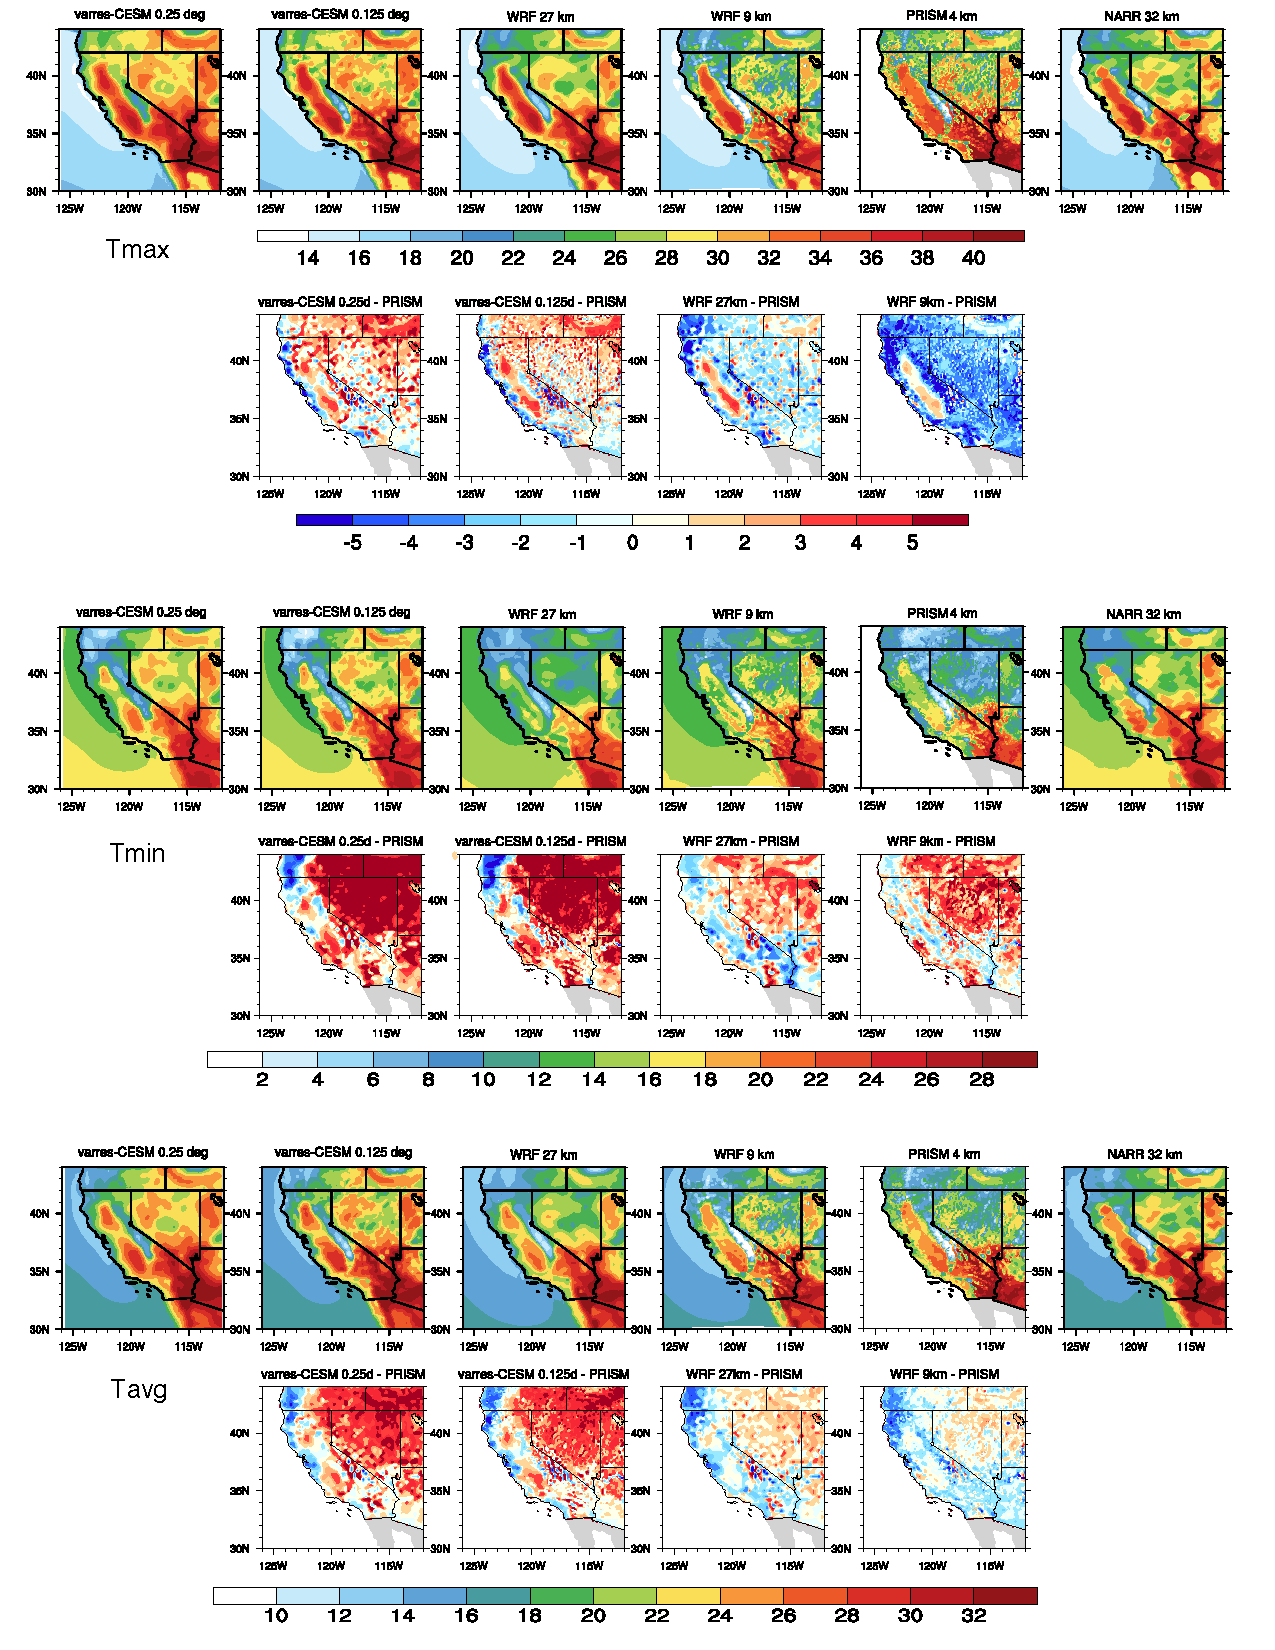
\includegraphics[width=6in]{t2_JJA.pdf}
\end{center}
\caption{JJA averaged daily T$_{max}$, T$_{min}$ and T$_{avg}$ from models and reference datasets, and differences (sharing the same legend) between model results and PRISM.} \label{fig:t2_JJA}
\end{figure}

%UW and Daymet are similar to PRISM, so only PRISM is presented here.

%Figure 5
\begin{figure}
\begin{center}
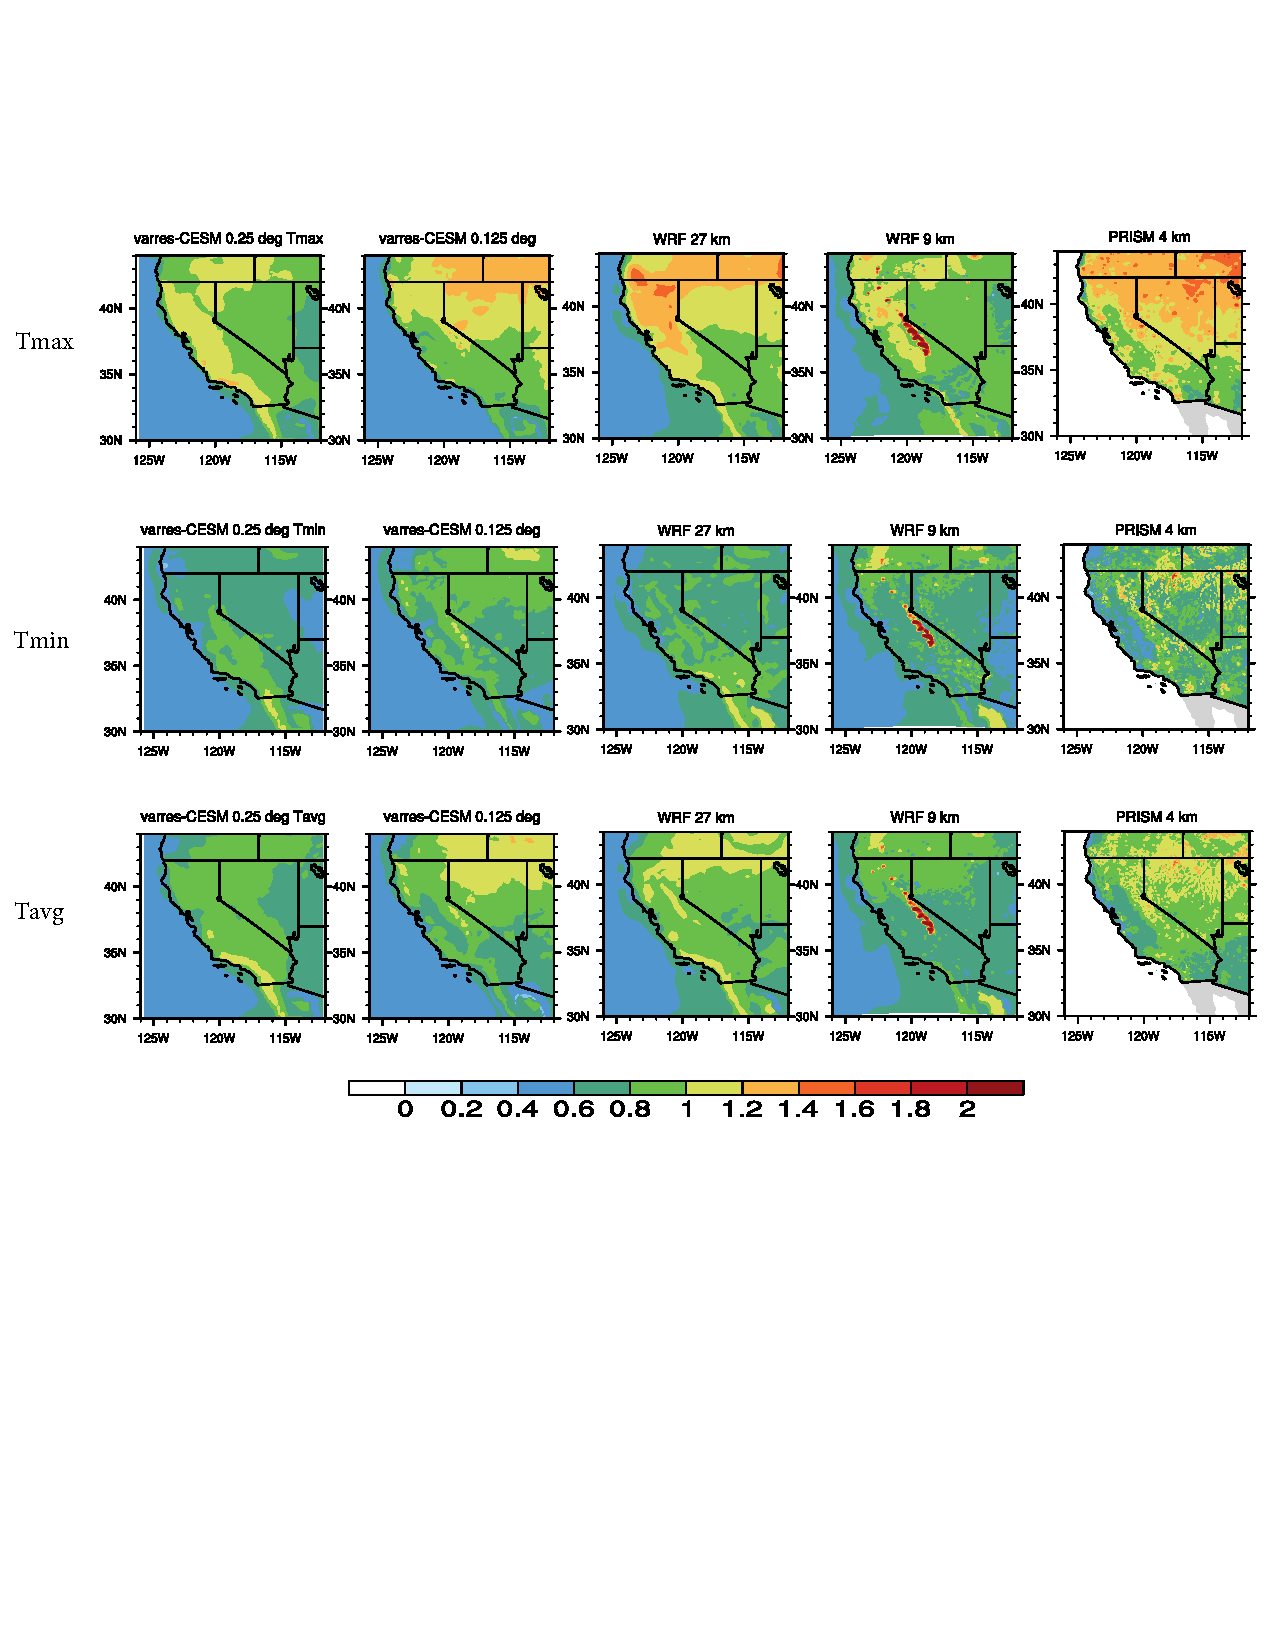
\includegraphics[width=6in]{t2_JJA_std.pdf}
\end{center}
\caption{Sample standard deviation of JJA average daily T$_{max}$, T$_{min}$ and T$_{avg}$ from model results and PRISM.} \label{fig:t2_JJA_std}
\end{figure}

%Figure 6
\begin{figure}
\begin{center}
\includegraphics[width=6in]{trd_t2avg_allzones.pdf}
\end{center}
\caption{Seasonal cycle of monthly-average T$_{avg}$ for each climate division. The shading corresponds to the 95\% confidence interval of PRISM and NARR. } \label{fig:trd_t2avg_allzones}
\end{figure}

%Figure 7
\begin{figure}
\begin{center}
\includegraphics[width=6in]{trd_t2avg_allzones_std.pdf}
\end{center}
\caption{Standard deviation values of monthly-average T$_{avg}$ for each climate division.} \label{fig:trd_t2avg_allzones_std}
\end{figure}

%Figure 8
\begin{figure}
\begin{center}
\includegraphics[width=6in]{PDF_t2max_allzones_JJA.pdf}
\end{center}
\caption{Frequency distribution of JJA daily T$_{max}$ over the simulation period 1980-2005.} \label{fig:PDF_t2max_allzones_JJA}
\end{figure}

%PRISM has no daily dataset for year 1980. And NARR is not presented here due to 

%Figure 9
\begin{figure}
\begin{center}
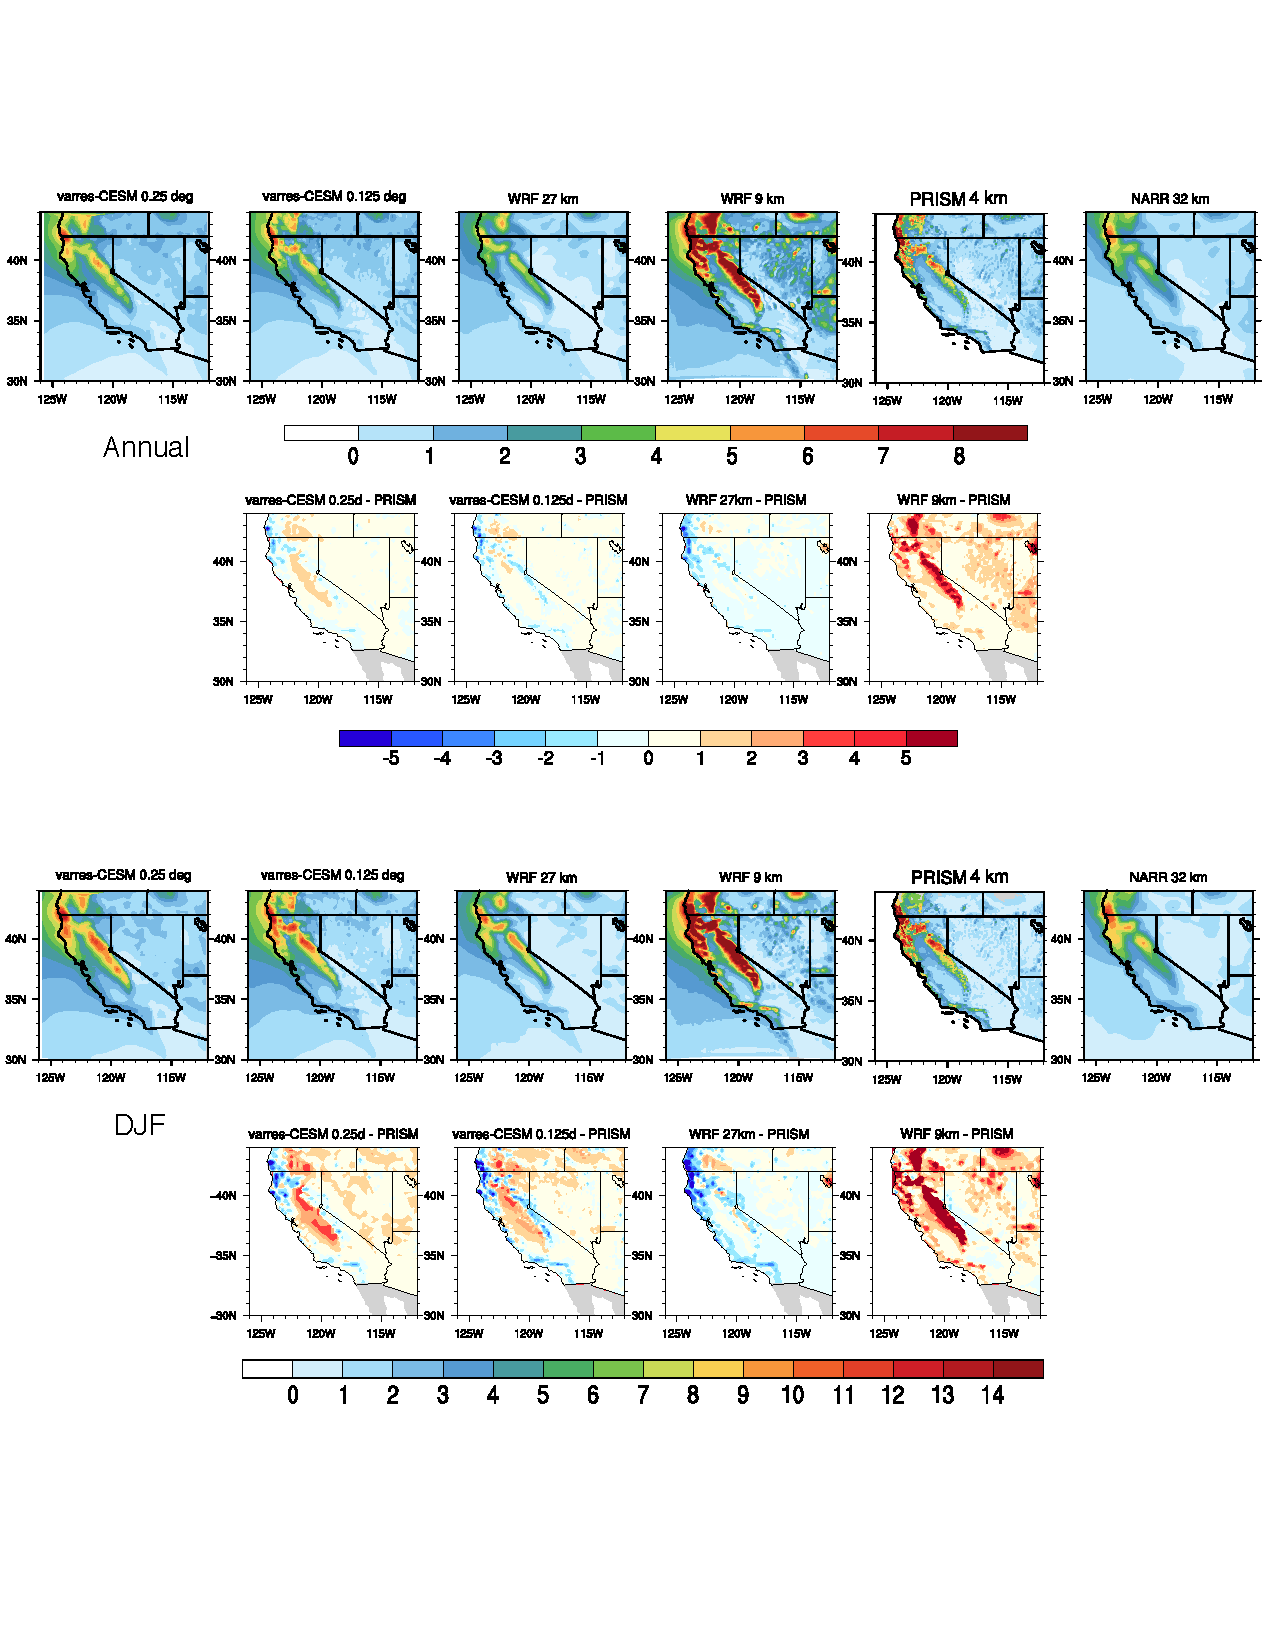
\includegraphics[width=6in]{pr_DJF_Annual.pdf}
\end{center}
\caption{Annual and DJF precipitation from model results and reference datasets, and differences (sharing the same legend) between model results and PRISM.} \label{fig:pr_DJF_Anuual}
\end{figure}

%Figure 10
\begin{figure}
\begin{center}
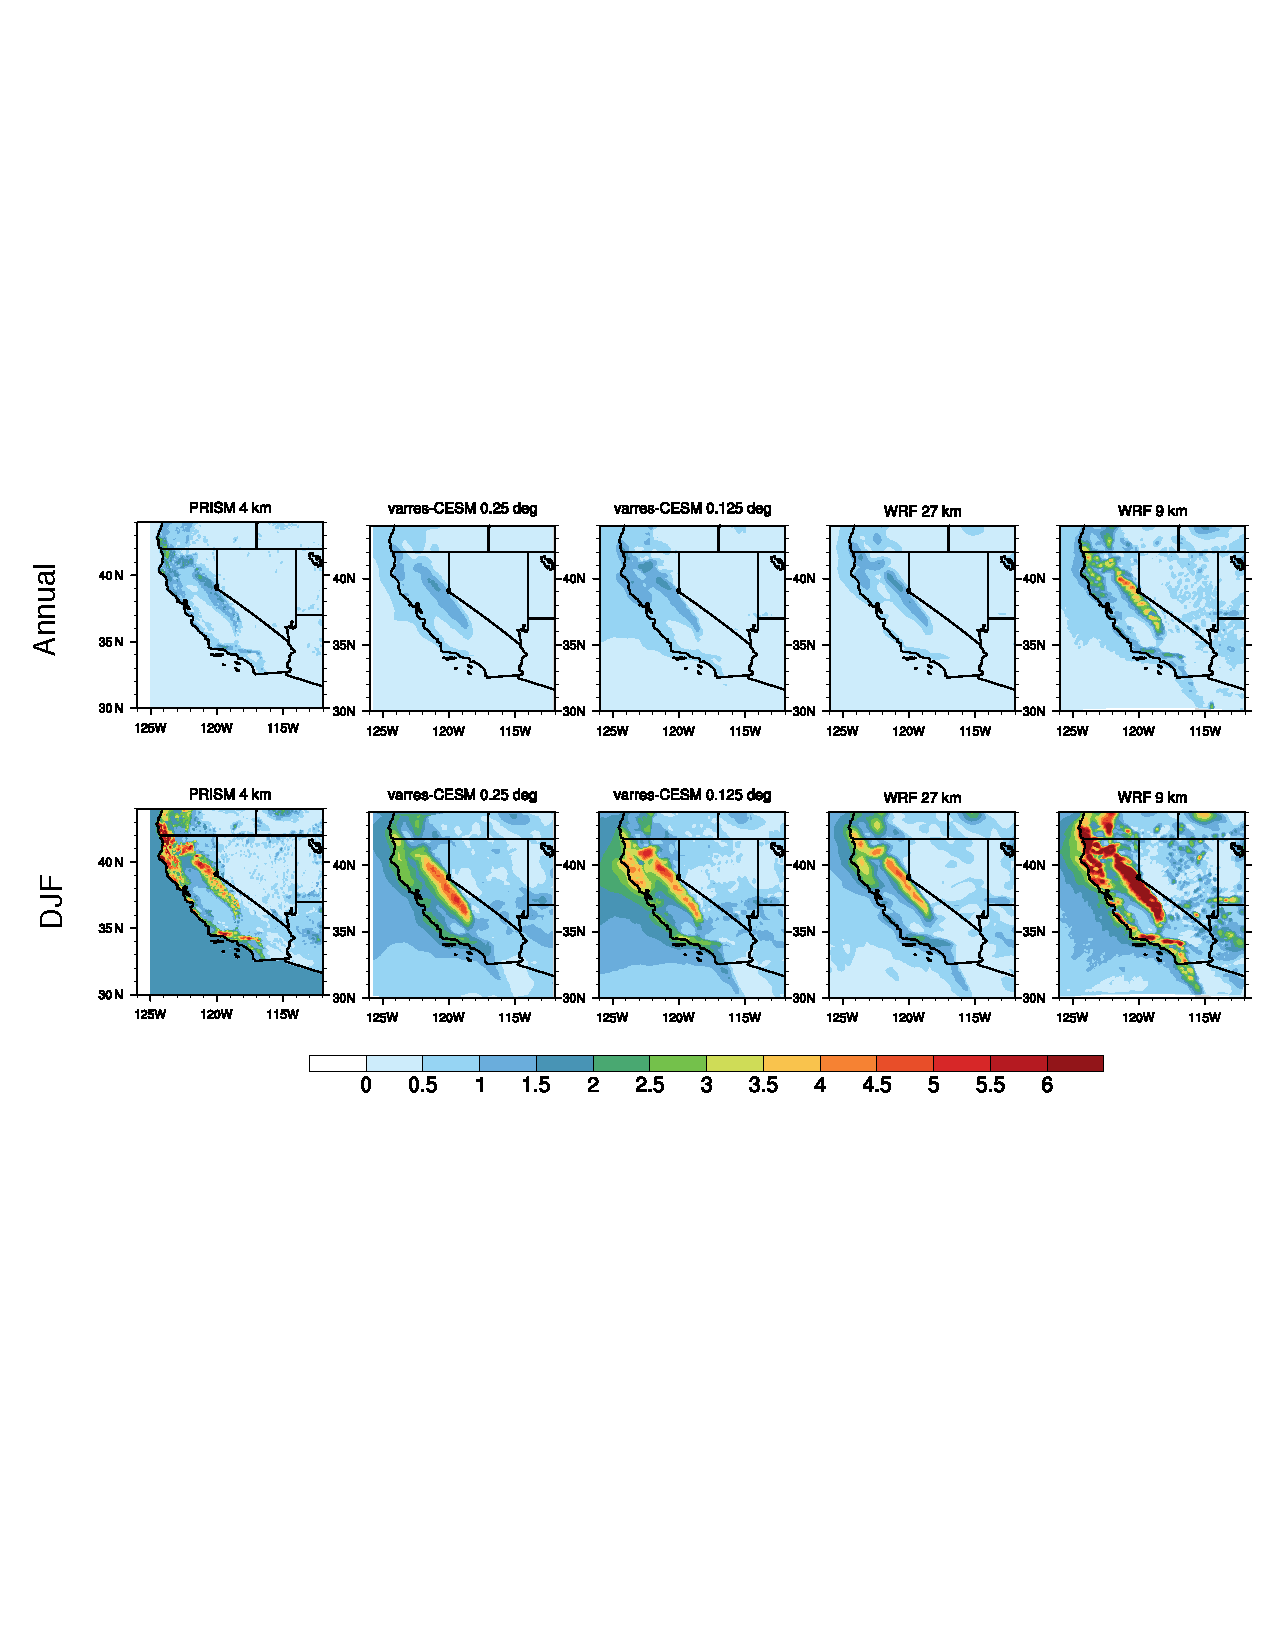
\includegraphics[width=6in]{pr_DJF_Annual_std.pdf}
\end{center}
\caption{Sample standard deviation of Annual and DJF precipitation from models and PRISM.} \label{fig:pr_DJF_Annual_std}
\end{figure}

%Figure 11
\begin{figure}
\begin{center}
\includegraphics[width=6in]{trd_pr_allzones.pdf}
\end{center}
\caption{As Figure 6, but for monthly-average total precipitation. The shading refers to the 95\% confidence interval of PRISM and UW.} \label{fig:trd_pr_allzones}
\end{figure}

%PRISM and UW are enough to represent the high-resolution gridded observations . So CPC and Daymet datasets are not displayed here.

%Figure 12
\begin{figure}
\begin{center}
\includegraphics[width=6in]{trd_pr_allzones_std.pdf}
\end{center}
\caption{As Figure 7, but for monthly-average total precipitation.} \label{fig:trd_pr_allzones_std}
\end{figure}

%Figure 13
\begin{figure}
\begin{center}
\includegraphics[width=6in]{PDF_pr_allzones_DJF.pdf}
\end{center}
\caption{As Figure 8, but for DJF Pr (note that the vertical scale is logarithmic).} \label{fig:PDF_pr_allzones_DJF}
\end{figure}

%Figure 14
\begin{figure}
\begin{center}
\includegraphics[width=6in]{taylor_diagram.pdf}
\end{center}
\caption{Taylor diagram of the annual climatology for the entire California region using the PRISM dataset as reference.} \label{fig:taylor_diagram}
\end{figure}


%Lastly, I think the paper should be re-read with the overall goal in mind. It seems like the goal is to demonstrate that VR-CESM performs as well as WRF in California. This should be kept in mind when you are discussing the results -- for example, if a bias exists in CAM, but is also seen in WRF, you should highlight that this likely represents a systematic issue with high-resolution models with respect to California. 

%add units for supplement

\end{document}
